\documentclass[12pt]{article}
\usepackage{graphicx} % Required for inserting images
% Language setting
% Replace english' with e.g. spanish' to change the document language
\usepackage[english]{babel}
\usepackage{booktabs}
\usepackage{mathtools}
\usepackage{subfig}
\usepackage[hidelinks]{hyperref}
\usepackage{caption}
\usepackage{blindtext}
\usepackage{graphicx}
\usepackage{cleveref}
\usepackage{setspace}
\usepackage{tikz}
\usepackage{placeins}  % in preamble
\usepackage{flafter}
% In your document
\FloatBarrier 
\usepackage{amsmath}
\usepackage{float}
\usepackage{multirow}
\usepackage{placeins}
\usepackage{hyperref}
% \usepackage{placeins} % for tables placement hbt!
\usepackage{float}
\usepackage[letterpaper,top=2cm,bottom=2cm,left=2cm,right=2cm,marginparwidth=1.75cm]{geometry}

\setlength{\arrayrulewidth}{0.5mm}
\setlength{\tabcolsep}{18pt}
\renewcommand{\arraystretch}{1.5}
\usepackage{tabularx, tabulary, longtable}
\usepackage{afterpage}
\usepackage{afterpage}
\usepackage{empheq}
\usepackage{tikz}
\usepackage{listings}
\usepackage{xcolor}
\usepackage[table]{xcolor}
\lstset{
    language=Matlab,
    basicstyle=\ttfamily\small,
    keywordstyle=\color{blue},
    commentstyle=\color{green},
    stringstyle=\color{red},
    numbers=left,
    numberstyle=\tiny\color{gray},
    stepnumber=1,
    numbersep=5pt,
    backgroundcolor=\color{white},
    showspaces=false,
    showstringspaces=false,
    showtabs=false,
    frame=single,
    rulecolor=\color{green},
    tabsize=2,
    captionpos=b,
    breaklines=true,
    breakatwhitespace=true,
    title=\lstname
}

\usetikzlibrary{shapes.geometric, arrows}
\usepackage{etoolbox}
\usepackage{amsmath}
\usepackage{subfig}
\usepackage[colorlinks=true, allcolors=blue]{hyperref}
\usepackage{authblk}
\usepackage{amssymb}
\usepackage{cite}
\usepackage{amsfonts}
\usepackage{amstext}
\usepackage{amsthm}
\usepackage{tikz}
\usepackage{listings}
\usepackage{xcolor}
\usetikzlibrary{shapes.geometric, arrows}
\usepackage{etoolbox}
\usepackage{subcaption}
\makeatletter
\patchcmd{\subsection}{\bfseries}{\itshape}{}{}
\patchcmd{\@sect}{\@addpunct.}{}{}{}
\makeatother
\newtheorem{theorem}{Theorem}
\newtheorem{remark}{Remark}[theorem]

% ---- Draft markup: new content added for the SciML extension is shown in red.
% Remove \new{} wrappers / newtext environments once coauthors approve the text.
\newcommand{\new}[1]{{\color{red}#1}}
\newenvironment{newtext}{\par\color{red}}{\par}

\title{\textcolor{Black}{\textbf{Comparative Analysis of Numerical Schemes for Two-Dimensional Dam-Break Problems with Source Terms under Different Initial Dam Breaking Conditions
}}}
\author[1]{Zahra}
\author[1]{M. Asif Farooq}
\author[2]{\textcolor{red}{Michael Ajao-Olarinoye}}
\author[1]{Firdos Khan}
\affil[1]{Department of Mathematics, School of Natural Sciences (SNS), National University of Sciences and Technology (NUST), Islamabad, Pakistan\newline
zahrasamad1998@gmail.com (zahra), asiffarooq.2007@gmail.com (M. Asif Farooq),
fkyousafzai@gmail.com (Firdos Khan)}
\affil[2]{\textcolor{red}{Centre for Computational Science and Mathematical Modelling, Coventry University, Coventry, United Kingdom\newline
ajaoolarinoyemichael@gmail.com (Michael Ajao-Olarinoye)}}
\begin{document}
\doublespacing
\maketitle
%\title{}
%\author[1]{Snabil Khan}
%\author[1]{Muhammad Asif Farooq}
%\affil[1]{Department of Mathematics, School of Natural Sciences, National University of Sciences and Technology, Islamabad, Pakistan}
\renewcommand\thesection{\arabic{section}}  % Ensures normal section numbering
\renewcommand\thesubsection{\thesection.\arabic{subsection}}  % Subsections as 1.1, 1.2, etc.
\section{Introduction}

\begin{newtext}
% ---- SCAFFOLD (new, in red): Introduction. Structure: motivation -> SWEs and
% shocks -> classical schemes -> SciML promise and failure modes -> positioning
% vs prior comparisons -> contributions -> outline. Replace bracketed TODOs.

The catastrophic failure of dams releases large volumes of water that propagate downstream as rapidly varying, highly unsteady free-surface flows, posing severe risks to infrastructure and human life. Accurate and fast simulation of dam-break wave propagation is therefore a cornerstone of hydraulic engineering, flood hazard assessment, and emergency response planning. The hydrodynamics of such events are described by the two-dimensional shallow water equations (SWEs), a nonlinear hyperbolic system obtained by depth-averaging the Navier--Stokes equations under a hydrostatic pressure assumption \cite{toro2001shockcapturing,kurganov2018finite}. A defining feature of this system is that discontinuities (shocks, hydraulic jumps) form in finite time even from smooth initial data, and realistic modeling must additionally account for bed-topography source terms and frictional resistance \cite{bermudez1994upwind,audusse2004fast}.

For decades, the standard tools for these problems have been shock-capturing finite difference and finite volume schemes: the classical Lax--Wendroff method \cite{lax1960systems}, Godunov-type methods built on exact or approximate Riemann solvers \cite{godunov1959difference,roe1981approximate,harten1983upstream,toro1994hllc}, and higher-order MUSCL-type reconstructions with slope limiters \cite{vanleer1979towards} advanced by strong-stability-preserving time integrators \cite{gottlieb2001strong}. These methods offer rigorous conservation and robust shock capturing, but their cost scales with grid resolution and the CFL constraint, which limits their use in real-time forecasting and ensemble-based risk assessment.

Scientific machine learning offers a complementary paradigm. Physics-informed neural networks (PINNs) \cite{raissi2019physics} parameterize the space-time solution with a neural network trained on the PDE residual, and have been applied to the SWEs in a growing body of work \cite{dazzi2024augmented,qi2024pinnswe,tian2025pinnswe,mumtaz2025dambreak,qi2025ndawl}. However, strong-form PINNs face well-documented difficulties on hyperbolic problems: the pointwise residual is ill-defined at discontinuities \cite{mao2020highspeed,oubarka2026wepinn}, the trained network does not enforce discrete conservation and can leak mass, and spectral bias drives solutions toward overly smooth, dissipative approximations of sharp fronts \cite{rahaman2019spectral}. Hybrid approaches that replace the strong-form residual with a discrete finite-volume residual restore conservation structure \cite{liu2026fvmpinn,wei2025ffvpinn,patsatzis2025gorinns,lichtle2025unfv,wu2025rimnet}, but their behavior across systematically varied dam-break initial conditions and topography source terms remains largely unexplored.

Several recent studies have compared neural solvers against classical schemes for dam-break flows. Mumtaz et al.~\cite{mumtaz2025dambreak} compared PINNs against a Lax--Wendroff baseline for 1D and 2D dam-break scenarios and found that PINNs reproduce the reference solutions with limited accuracy, improving when numerical solutions are injected into training. Tian et al.~\cite{tian2025pinnswe} benchmarked PINNs for the 2D SWEs with topography and rainfall source terms against an HLL scheme, finding errors concentrated at shock and rarefaction fronts. Qi et al.~\cite{qi2024pinnswe} compared data-free PINNs against a finite-volume solver, including a real-world flood event. Liu \cite{liu2026fvmpinn} showed that a finite-volume-informed PINN loss produces a rugged landscape in which physics-only training collapses to a spurious low-momentum state unless sparse data guidance is supplied. [TODO: sharpen positioning after final experiments -- what distinguishes this study is the systematic crossing of \emph{initial-condition geometry} (six profiles), \emph{classical scheme family} (LW / HLL / MUSCL--Rusanov), and \emph{neural formulation} (primitive vs.\ conservative strong-form PINN, and an FVM-informed PINN with a discrete HLLC residual), all over a non-flat bed.]

The contributions of this work are:
\begin{enumerate}
  \item A benchmark matrix of six 2D dam-break initial-condition geometries (step, rectangular, circular, Gaussian, parabolic, triangular) over a Gaussian-hump bed topography, solved with three classical schemes (Lax--Wendroff, HLL, MUSCL--Rusanov) that serve as reference solutions.
  \item A systematic evaluation of strong-form PINNs in both primitive $(h,u,v)$ and conservative $(h,hu,hv)$ formulations on this benchmark matrix, quantifying accuracy, mass-conservation error, and shock-front smearing as a function of initial-condition geometry.
  \item A finite-volume-informed PINN whose loss is the discrete-consistency residual of a differentiable HLLC/SSP--RK solver step, with positivity of depth enforced by construction through a softplus reparameterization, and an ablation of sparse-data guidance.
  \item A quantitative comparison of all methods with respect to accuracy against the reference solutions, conservation, shock-front position error, and computational cost. [TODO: finalize once runs complete.]
\end{enumerate}

The remainder of the paper is organized as follows. Section 2 reviews related work. Section 3 presents the governing equations, the classical numerical schemes, the benchmark initial conditions, and the neural network formulations. Section 4 reports results for the classical schemes and the SciML comparison. Section 5 discusses implications and limitations, and Section 6 concludes.
\end{newtext}

\begin{newtext}
% ---- SCAFFOLD (new, in red): Related Work section.
\section{Related Work}

\subsection{Classical shock-capturing schemes for dam-break flows}
Godunov's method \cite{godunov1959difference} and its descendants compute intercell fluxes from (approximate) Riemann solutions. The Roe linearization \cite{roe1981approximate} resolves isolated shocks sharply but requires entropy fixes; the HLL solver \cite{harten1983upstream} is robust and positivity-preserving but dissipative at contact waves, a deficiency corrected by HLLC \cite{toro1994hllc}. The Rusanov flux \cite{rusanov1961calculation} is the simplest and most dissipative member of this family. Second-order accuracy is obtained through MUSCL reconstruction with slope limiters \cite{vanleer1979towards}, and higher-order alternatives such as WENO-Z \cite{borges2008improved} trade cost for resolution. For the SWEs specifically, source-term treatment matters as much as the flux: well-balanced schemes preserving lake-at-rest equilibria \cite{bermudez1994upwind,audusse2004fast} and positivity-preserving wet/dry treatments \cite{xing2010positivity} are standard requirements; see \cite{kurganov2018finite} for a survey. Verification practice relies on analytic solutions \cite{stoker1957water,delestre2013swashes} and established 2D benchmarks, including the partial dam-breach basin of Fennema and Chaudhry \cite{fennema1990explicit}, the dam break over three humps \cite{kawahara1986finite}, and laboratory experiments with an isolated obstacle \cite{soaresfrazao2007experimental}.

\subsection{Physics-informed neural networks for the SWEs}
PINNs \cite{raissi2019physics} minimize a composite loss over PDE residuals, initial and boundary conditions, with derivatives obtained by automatic differentiation. Applied to hyperbolic systems, strong-form PINNs struggle at discontinuities, where the classical derivatives diverge \cite{mao2020highspeed}; spectral bias further favors smooth, low-frequency solutions \cite{rahaman2019spectral}, so dam-break fronts are systematically smeared. For the SWEs, Dazzi \cite{dazzi2024augmented} recast the topography as an augmented conserved variable; Qi et al.~\cite{qi2024pinnswe} trained data-free fully-connected and convolutional PINNs against finite-volume references including a real flood; Tian et al.~\cite{tian2025pinnswe} added terrain and rainfall source terms with an HLL baseline and reported an entropy-conditioned variant failing on the dam-break case; NDAWL-PINN \cite{qi2025ndawl} addresses the multi-term loss-balancing pathology through non-dimensionalization and multi-task weighting; and Mumtaz et al.~\cite{mumtaz2025dambreak} systematically compared PINNs against Lax--Wendroff across dam geometries and initial water-height profiles. Weak-form and entropy-based reformulations \cite{oubarka2026wepinn} replace the pointwise residual with integral constraints that remain well-defined across shocks.

\subsection{Finite-volume-informed and hybrid neural solvers}
A second line of work embeds discrete conservation structure into the learning problem. Liu \cite{liu2026fvmpinn} evaluates the loss through a differentiable well-balanced Roe-type finite-volume discretization on unstructured meshes and documents a rugged loss landscape in which physics-only training collapses to a trivial low-momentum state, remedied by sparse data guidance. FFV-PINN \cite{wei2025ffvpinn} uses a simplified finite-volume discretization of the convective terms with residual correction to stabilize and accelerate training. GoRINNs \cite{patsatzis2025gorinns} and (U)NFV \cite{lichtle2025unfv} learn flux functions or update rules inside Godunov-type schemes, preserving conservation by construction, while RimNet \cite{wu2025rimnet} replaces the Riemann solver with a neural surrogate inside a finite-volume scheme, generalizing across dam-break initial conditions at reduced runtime. The FVM-informed PINN in this study belongs to this family: the network is trained so that its predicted states are consistent with a differentiable HLLC/SSP--RK solver step (Sect.~3), rather than with a pointwise strong-form residual.

\subsection{Neural operators}
Neural operators learn mappings between function spaces, so a trained model generalizes across initial conditions without retraining: DeepONet \cite{lu2021deeponet} and its physics-informed variant \cite{wang2021pideeponet}, the Fourier neural operator \cite{li2021fourier,kovachki2023neuraloperator}, and physics-informed neural operators \cite{li2024pino} are the principal architectures, with applications to computational hydraulics and flood modeling \cite{liu2026hydraulics,keppler2025pinoswe,secchi2026debrisflow}. Spectral truncation in FNO-type models, however, acts as a low-pass filter that smears shock fronts over long rollouts; multi-scale remedies include local-global operators \cite{wang2026lgno}, dual-channel wavelet operators \cite{lu2026dcmawno}, and latent-space operator learning \cite{kontolati2024latent}. Operator learning is outside the scope of the present single-instance comparison, but constitutes the natural extension of the FVM-informed training studied here. [TODO: decide whether to keep this subsection or compress into one paragraph, depending on venue page limits.]
\end{newtext}

\section{Problem Setup}

In this section, the two dimensional shallow water equations (SWEs) and the numerical schemes used to solve them are presented. The governing equations used in this study are the same as the standard equations, but they include bed topography source terms. The reference solutions are computed using the three numerical schemes: the Lax–Wendroff (LW) scheme, the Harten–Lax–van Leer (HLL) approximate Riemann solver, and the MUSCL-Rusanov (MUSCL-RS) scheme. The six dam-break scenarios examined include Step, Rectangular, Circular, Gaussian, Parabolic and Triangular water height profiles. These benchmark problems are described in detail in Sect.~2.3. The numerical solutions are then evaluated and compared with respect to the performance, accuracy and shock capturing ability of the numerical schemes considered. \new{In addition, Sect.~2.4 introduces the scientific machine learning models evaluated against these reference solutions: strong-form physics-informed neural networks in primitive and conservative formulations, and a finite-volume-informed PINN trained on the discrete residual of a differentiable HLLC solver step.}

\subsection{Governing Equations}
The mathematical model governing the hydrodynamic flow in this study is the two-dimensional (2D) Shallow Water Equations (SWEs). The equations are obtained by hydrostatic pressure distribution, by neglecting the vertical acceleration, and by considering the fluid density as constant and by depth integrating the Navier-Stokes equations. The SWEs are hyperbolic conservation laws which are in effect for the propagation of water waves in domains where the horizontal length scale is much greater than the water depth.The present study is based on the standard formulation of the equations to which a source term vector $\mathbf{S}$, representing the effects of bottom topography (bed slope), and bed friction are added. These source terms are important to include in order to simulate a realistic flood, as they describe the effects of topography and resistance to flow.

\begin{equation}
\frac{\partial \mathbf{U}}{\partial t}
+\frac{\partial \mathbf{F}(\mathbf{U})}{\partial x}
+\frac{\partial \mathbf{G}(\mathbf{U})}{\partial y}
=\mathbf{S}(x,y,t,\mathbf{U}),
\label{eq:swe}
\end{equation}

where $t$ denotes time, $x$ and $y$ are the spatial coordinates, $\mathbf{U}$ is the vector of conserved variables, $\mathbf{F}$ and $\mathbf{G}$ are the flux vectors in the $x$- and $y$-directions, respectively, and $\mathbf{S}$ is the source term vector.

The vectors $\mathbf{U}$, $\mathbf{F}$, and $\mathbf{G}$ are defined as

\begin{equation}
\mathbf{U}=
\begin{bmatrix}
h \\
hu \\
hv
\end{bmatrix},
\qquad
\mathbf{F}(\mathbf{U})=
\begin{bmatrix}
hu \\
hu^{2}+\dfrac{1}{2}gh^{2} \\
huv
\end{bmatrix},
\qquad
\mathbf{G}(\mathbf{U})=
\begin{bmatrix}
hv \\
huv \\
hv^{2}+\dfrac{1}{2}gh^{2}
\end{bmatrix}.
\label{eq:flux}
\end{equation}


These are the expressions for the water depth $h$, the depth-averaged velocity components, $u$ and $v$ in the $x$ and $y$ directions, respectively, and $g$ the gravitational acceleration. The quantities $hu$ and $hv$ are the momentum fluxes per unit width.

The source term vector $\mathbf{S}$ represents the forces on the flow other than its internal forces. The influence of bed slope (topography) and bed friction (Manning roughness) are taken into account in the present study. As a result, $\mathbf{S}$ is given by

\begin{equation}
\mathbf{S}=
\begin{bmatrix}
0 \\
-gh\displaystyle\frac{\partial Z}{\partial x}
-\displaystyle\frac{gn^{2}u\sqrt{u^{2}+v^{2}}}{h^{4/3}} \\
-gh\displaystyle\frac{\partial Z}{\partial y}
-\displaystyle\frac{gn^{2}v\sqrt{u^{2}+v^{2}}}{h^{4/3}}
\end{bmatrix}.
\label{eq:source}
\end{equation}

In this equation $Z(x,y)$ is the bed elevation and $n$ is the Manning roughness coefficient. The first term of $\mathbf{S}$ is null, meaning that the transfer of mass from an external source (rainfall and/or infiltration) is not taken into account in the continuity equation. The second term and third term are the terms that represent the momentum source terms in the $x$ and $y$ directions, respectively.

The terms $-gh\frac{\partial Z}{\partial x}$, $-gh\frac{\partial Z}{\partial y}$ represent the driving forces due to the sloping bed, where $g$ and $h$ are the magnitude of gravity and the height above sea level, respectively.
The terms involving $n$ represent the losses due to the friction between the bed and the water.

For the present numerical study, the Manning coefficient is assumed as $n=0$. The friction terms then drop off and the source term vector becomes

\begin{equation}
\mathbf{S}=
\begin{bmatrix}
0 \\
-gh\displaystyle\frac{\partial Z}{\partial x} \\
-gh\displaystyle\frac{\partial Z}{\partial y}
\end{bmatrix}.
\label{eq:simplifiedsource}
\end{equation}

\subsection{Numerical Schemes}

In this study, three distinct numerical schemes are employed to solve the two-dimensional shallow water equations with source terms. These schemes are the Lax--Wendroff (LW) method, the Harten--Lax--van Leer (HLL) approximate Riemann solver, and the MUSCL scheme with third-order Strong Stability Preserving Runge--Kutta (SSP--RK3) time integration. Each scheme is described in detail in the following subsections.

\subsubsection{Lax--Wendroff Scheme}

The Lax--Wendroff scheme is a second-order accurate finite difference method that employs a predictor--corrector approach. It is widely used for solving hyperbolic conservation laws due to its ability to capture wave propagation with reasonable accuracy while maintaining computational efficiency.

The scheme follows a two-step procedure at each time level.

\paragraph{Predictor Step}

The intermediate solution at the half time level $t^{n+\frac{1}{2}}$ is computed as

\begin{equation}
U_{i,j}^{\,n+\frac{1}{2}}
=
U_{i,j}^{\,n}
-\frac{\Delta t}{2\Delta x}
\left(
F_{i+1,j}^{\,n}
-
F_{i-1,j}^{\,n}
\right)
-\frac{\Delta t}{2\Delta y}
\left(
G_{i,j+1}^{\,n}
-
G_{i,j-1}^{\,n}
\right)
+\frac{\Delta t}{2}S_{i,j}^{\,n},
\end{equation}

where $U_{i,j}^{\,n+\frac{1}{2}}$ denotes the predicted conservative variables at the half time level, and $S_{i,j}^{\,n}$ represents the source term vector associated with bed topography.

The source term vector is given by

\begin{equation}
S=
\begin{bmatrix}
0 \\
-gh\frac{\partial Z}{\partial x} \\
-gh\frac{\partial Z}{\partial y}
\end{bmatrix},
\end{equation}

where $Z(x,y)$ denotes the bed elevation.

\paragraph{Flux Evaluation}

After computing the intermediate variables, the flux vectors are evaluated at the half time level as

\begin{equation}
F^{\,n+\frac{1}{2}}
=
\begin{bmatrix}
hu \\
hu^{2}+\frac{1}{2}gh^{2} \\
huv
\end{bmatrix},
\qquad
G^{\,n+\frac{1}{2}}
=
\begin{bmatrix}
hv \\
huv \\
hv^{2}+\frac{1}{2}gh^{2}
\end{bmatrix}.
\end{equation}

\paragraph{Corrector Step}

The full time-step update is given by

\begin{equation}
U_{i,j}^{n+1}
=
U_{i,j}^{n}
-
\frac{\Delta t}{\Delta x}
\left(
F_{i+\frac{1}{2},j}^{\,n+\frac{1}{2}}
-
F_{i-\frac{1}{2},j}^{\,n+\frac{1}{2}}
\right)
-
\frac{\Delta t}{\Delta y}
\left(
G_{i,j+\frac{1}{2}}^{\,n+\frac{1}{2}}
-
G_{i,j-\frac{1}{2}}^{\,n+\frac{1}{2}}
\right)
+
\Delta t\,S_{i,j}^{\,n+\frac{1}{2}}.
\end{equation}

The scheme achieves second-order accuracy in both space and time. However, it may produce spurious oscillations near steep gradients or discontinuities, which is a known limitation of this method.

\subsubsection{Harten--Lax--van Leer (HLL) Scheme}

The HLL scheme is an approximate Riemann solver that computes intercell fluxes based on wave-speed estimates. It is a Godunov-type finite volume method that provides robust solutions for hyperbolic conservation laws, particularly in the presence of shocks and discontinuities.

For the $x$-direction, the HLL flux between the left and right states, denoted by $\mathbf{U}_L$ and $\mathbf{U}_R$, respectively, is given by

\begin{equation}
\mathbf{F}_{i+\frac{1}{2}}^{HLL}=
\begin{cases}
\mathbf{F}_L, & \text{if } S_L \geq 0, \\[2mm]
\dfrac{S_R\mathbf{F}_L-S_L\mathbf{F}_R+S_LS_R(\mathbf{U}_R-\mathbf{U}_L)}
{S_R-S_L}, & \text{if } S_L<0<S_R, \\[3mm]
\mathbf{F}_R, & \text{if } S_R \leq 0.
\end{cases}
\end{equation}

where the wave speeds are estimated as

\begin{equation}
S_L=\min\left(u_L-c_L,\,u_R-c_R\right),
\end{equation}

\begin{equation}
S_R=\max\left(u_L+c_L,\,u_R+c_R\right),
\end{equation}

where

\begin{equation}
c_L=\sqrt{gh_L},
\qquad
c_R=\sqrt{gh_R},
\end{equation}

and

\begin{equation}
u_L=\frac{(hu)_L}{h_L},
\qquad
u_R=\frac{(hu)_R}{h_R}.
\end{equation}

Similarly, for the $y$-direction, the HLL flux is given by

\begin{equation}
\mathbf{G}_{j+\frac{1}{2}}^{HLL}=
\begin{cases}
\mathbf{G}_B, & \text{if } S_L \geq 0, \\[2mm]
\dfrac{S_R\mathbf{G}_B-S_L\mathbf{G}_T+S_LS_R(\mathbf{U}_T-\mathbf{U}_B)}
{S_R-S_L}, & \text{if } S_L<0<S_R, \\[3mm]
\mathbf{G}_T, & \text{if } S_R \leq 0.
\end{cases}
\end{equation}

where the wave speeds in the $y$-direction are estimated as

\begin{equation}
S_L=\min\left(v_B-c_B,\,v_T-c_T\right),
\end{equation}

\begin{equation}
S_R=\max\left(v_B+c_B,\,v_T+c_T\right),
\end{equation}

with

\begin{equation}
c_B=\sqrt{gh_B},
\qquad
c_T=\sqrt{gh_T}.
\end{equation}

The source term is incorporated explicitly through the semi-discrete formulation

\begin{equation}
\frac{\partial \mathbf{U}}{\partial t}
=
-\frac{\partial \mathbf{F}}{\partial x}
-\frac{\partial \mathbf{G}}{\partial y}
+\mathbf{S}.
\end{equation}

The spatial derivatives are approximated using the HLL fluxes, whereas the temporal integration is performed using the SSP--RK3 scheme described in the next subsection.

\subsubsection{MUSCL Scheme with SSP--RK3 Time Integration}

The \textbf{Monotonic Upstream-centered Scheme for Conservation Laws (MUSCL)} is a second-order spatial reconstruction technique that improves the accuracy of the finite volume method while preserving monotonicity near discontinuities. In the present work, the MUSCL scheme is coupled with the Minmod slope limiter, the Rusanov (Local Lax--Friedrichs) numerical flux, and the third-order Strong Stability Preserving Runge--Kutta (SSP--RK3) method for time integration.

\paragraph{Spatial Reconstruction}

Within the finite volume framework, only the cell-averaged conservative variables are stored. Therefore, the left and right states at each cell interface are reconstructed using the MUSCL approach as

\begin{equation}
U_{i+\frac{1}{2}}^{L}
=
U_i
+
\frac{1}{2}
\Delta x
\,\Delta U_i,
\label{eq:MUSCL_left}
\end{equation}

\begin{equation}
U_{i+\frac{1}{2}}^{R}
=
U_{i+1}
-
\frac{1}{2}
\Delta x
\,\Delta U_{i+1},
\label{eq:MUSCL_right}
\end{equation}

where the limited slope is computed using the Minmod limiter

\begin{equation}
\Delta U_i
=
\operatorname{minmod}
\left(
\frac{U_i-U_{i-1}}{\Delta x},
\frac{U_{i+1}-U_i}{\Delta x}
\right).
\label{eq:slope}
\end{equation}

The Minmod function is defined as

\begin{equation}
\operatorname{minmod}(a,b)
=
\frac{1}{2}
\left[
\operatorname{sign}(a)
+
\operatorname{sign}(b)
\right]
\min
\left(
|a|,
|b|
\right).
\label{eq:minmod}
\end{equation}

The same reconstruction procedure is applied independently in both the $x$- and $y$-directions.

\paragraph{Rusanov Numerical Flux}

After reconstructing the left and right interface states, the physical fluxes are evaluated and the numerical flux at each interface is computed using the Rusanov (Local Lax--Friedrichs) flux

\begin{equation}
F_{i+\frac{1}{2}}
=
\frac{1}{2}
\left(
F_L+F_R
\right)
-
\frac{1}{2}
\alpha
\left(
U_R-U_L
\right),
\label{eq:rusanov}
\end{equation}

where

\begin{equation}
\alpha
=
\max
\left(
|u_L|+c_L,\,
|u_R|+c_R
\right),
\label{eq:alpha}
\end{equation}

denotes the maximum local wave speed, with

\begin{equation}
c=\sqrt{gh}.
\label{eq:wavespeed}
\end{equation}

Similarly, the numerical flux in the $y$-direction is evaluated as

\begin{equation}
G_{j+\frac{1}{2}}
=
\frac{1}{2}
\left(
G_B+G_T
\right)
-
\frac{1}{2}
\alpha_y
\left(
U_T-U_B
\right),
\label{eq:rusanov_y}
\end{equation}

where

\begin{equation}
\alpha_y
=
\max
\left(
|v_B|+c_B,\,
|v_T|+c_T
\right).
\label{eq:alpha_y}
\end{equation}

\paragraph{Semi-discrete Finite Volume Formulation}

After computing the numerical fluxes, the governing shallow water equations are transformed into the following semi-discrete finite volume form

\begin{equation}
\frac{dU_{i,j}}{dt}
=
-
\frac{
F_{i+\frac{1}{2},j}
-
F_{i-\frac{1}{2},j}
}{\Delta x}
-
\frac{
G_{i,j+\frac{1}{2}}
-
G_{i,j-\frac{1}{2}}
}{\Delta y}
+
S_{i,j}.
\label{eq:semidiscrete}
\end{equation}

The spatial discretization operator is denoted by

\begin{equation}
R(U)
=
-
\frac{
F_{i+\frac{1}{2},j}
-
F_{i-\frac{1}{2},j}
}{\Delta x}
-
\frac{
G_{i,j+\frac{1}{2}}
-
G_{i,j-\frac{1}{2}}
}{\Delta y}
+
S_{i,j}.
\label{eq:residual}
\end{equation}

\paragraph{SSP--RK3 Time Integration}

The semi-discrete finite volume system is advanced in time using the third-order Strong Stability Preserving Runge--Kutta (SSP--RK3) scheme.

\textbf{Stage 1}

\begin{equation}
U^{(1)}
=
U^{n}
+
\Delta t\,R(U^{n}),
\label{eq:rk3_stage1}
\end{equation}

\textbf{Stage 2}

\begin{equation}
U^{(2)}
=
\frac{3}{4}U^{n}
+
\frac{1}{4}
\left[
U^{(1)}
+
\Delta t\,R(U^{(1)})
\right],
\label{eq:rk3_stage2}
\end{equation}

\textbf{Stage 3}

\begin{equation}
U^{n+1}
=
\frac{1}{3}U^{n}
+
\frac{2}{3}
\left[
U^{(2)}
+
\Delta t\,R(U^{(2)})
\right].
\label{eq:rk3_stage3}
\end{equation}

The MUSCL scheme is a second-order finite-volume reconstruction method in which piecewise linear states are constructed from cell averages using a slope limiter. In this work, the Minmod limiter is employed to suppress spurious oscillations near discontinuities, while intercell fluxes are evaluated using the Rusanov (local Lax–Friedrichs) flux. The resulting semi-discrete system is advanced in time using the SSP–RK3 method, with the spatial residual recomputed at each Runge–Kutta stage.
\paragraph{Boundary Conditions:}

Reflective boundary conditions are imposed along all domain boundaries. The water depth is extrapolated using zero-gradient conditions, while the normal momentum component is reflected and the tangential momentum component is extrapolated with zero-gradient conditions.

\subsection{Initial Conditions for Dam-Break Scenarios}

In this study, six distinct initial water height profiles are considered to evaluate the performance of the numerical schemes. These profiles represent different dam-break configurations, ranging from simple discontinuous jumps to smooth Gaussian and geometric shapes. In all cases, the dam is assumed to be instantaneously removed at $t=0$, initiating wave propagation. The initial velocity is set to zero throughout the computational domain, i.e.,

\begin{equation}
u(x,y,0)=0,
\qquad
v(x,y,0)=0.
\end{equation}

The computational domain is taken as a square region of size

\begin{equation}
L_x \times L_y =100\times100~\mathrm{m}^2.
\end{equation}

The bed topography is prescribed as a Gaussian hump:

\begin{equation}
Z(x,y)=2.0\exp\left(
-\frac{(x-50)^2+(y-50)^2}{200}
\right).
\end{equation}

The gravitational acceleration is set to $g=2~\mathrm{m/s^2}$, while the Manning friction coefficient is taken as $n=0$.

\subsubsection{Variant 1: Step (Simple) Dam-Break}

This configuration represents the classical dam-break problem extended to two dimensions. The initial water height is defined as

\begin{equation}
h(x,y,0)=
\begin{cases}
h_l=10.0~\mathrm{m}, & \text{if } x\leq 50~\mathrm{m},\\
h_r=1.0~\mathrm{m}, & \text{if } x>50~\mathrm{m}.
\end{cases}
\end{equation}

This setup creates a sharp discontinuity at $x=50~\mathrm{m}$, producing a shock wave propagating to the right and a rarefaction wave propagating to the left after dam removal.

\subsubsection{Variant 2: Rectangular Dam-Break}

In this case, a rectangular region of high water is initially confined within the computational domain. The initial condition is given by

\begin{equation}
h(x,y,0)=
\begin{cases}
h_{\mathrm{in}}=5.0~\mathrm{m},
& \text{if } 30\leq x\leq70~\mathrm{m}
\text{ and }30\leq y\leq70~\mathrm{m},\\
h_{\mathrm{out}}=0.2~\mathrm{m},
& \text{otherwise}.
\end{cases}
\end{equation}

This configuration models the sudden release of water from a rectangular reservoir, leading to complex wave interactions at the corners and edges.

\subsubsection{Variant 3: Circular Dam-Break}

The circular dam configuration consists of a cylindrical water column centered within the domain. The initial water height is prescribed as

\begin{equation}
h(x,y,0)=
\begin{cases}
h_{\mathrm{in}}=10.0~\mathrm{m},
& \text{if }
\sqrt{(x-50)^2+(y-50)^2}\leq R,\\
h_{\mathrm{out}}=1.0~\mathrm{m},
& \text{otherwise},
\end{cases}
\end{equation}

where $R=20~\mathrm{m}$ denotes the radius of the circular dam.

Following dam removal, a radially symmetric wave propagates outward, providing an effective benchmark for assessing the ability of numerical schemes to capture circular shock fronts.

\subsubsection{Variant 4: Gaussian Dam-Break}

Unlike the previous discontinuous profiles, the Gaussian initial condition represents a smooth and continuous water surface. The initial water height is defined as

\begin{equation}
h(x,y,0)
=
h_{\mathrm{peak}}
\exp\left(
-\frac{(x-x_c)^2+(y-y_c)^2}
{2\sigma^2}
\right),
\end{equation}

where

\begin{itemize}
\item $h_{\mathrm{peak}}=10.0~\mathrm{m}$ is the maximum water height,
\item $(x_c,y_c)=(50.0,50.0)~\mathrm{m}$ denotes the center of the domain,
\item $\sigma=10.0~\mathrm{m}$ is the standard deviation controlling the spread of the Gaussian profile.
\end{itemize}

This smooth profile allows the evaluation of numerical schemes in the absence of sharp gradients and tests their ability to preserve the shape and amplitude of smooth waves.

\subsubsection{Variant 5: Parabolic Dam-Break}

The parabolic dam configuration represents a curved dam structure. The upper and lower boundaries of the parabolic region are defined by

\begin{equation}
y_{\mathrm{top}}(x)
=
y_c+w-a(x-x_c)^2,
\end{equation}

\begin{equation}
y_{\mathrm{bottom}}(x)
=
y_{\mathrm{top}}(x)-t,
\end{equation}

where the initial water height is prescribed as

\begin{equation}
h(x,y,0)=
\begin{cases}
h_{\mathrm{in}}=10.0~\mathrm{m},
& \text{if }
y_{\mathrm{bottom}}(x)
\leq y \leq
y_{\mathrm{top}}(x),\\
h_{\mathrm{out}}=1.0~\mathrm{m},
& \text{otherwise}.
\end{cases}
\end{equation}

The parameters used are

\begin{equation}
(x_c,y_c)=(50.0,50.0)~\mathrm{m},
\qquad
a=0.03,
\qquad
w=15.0~\mathrm{m},
\qquad
t=8.0~\mathrm{m}.
\end{equation}

This configuration tests the ability of numerical schemes to handle curved boundaries and non-rectangular geometries.

\subsubsection{Variant 6: Triangular (Equilateral) Dam-Break}

The initial water height profile is defined by an equilateral triangle centered at

\begin{equation}
(x_c,y_c)=(50.0,50.0)~\mathrm{m},
\end{equation}

with side length

\begin{equation}
s=40.0~\mathrm{m}.
\end{equation}

The height of the triangle is given by

\begin{equation}
h_{\mathrm{tri}}
=
\frac{\sqrt{3}}{2}s
=
34.64~\mathrm{m}.
\end{equation}

The three vertices of the triangular region are located at

\begin{align}
\text{Apex (Top):}\qquad
&(x_c,\; y_c+\tfrac{h_{\mathrm{tri}}}{3})
=(50.0,\;61.55), \\
\text{Left Base Vertex:}\qquad
&(x_c-\tfrac{s}{2},\;
y_c-\tfrac{2h_{\mathrm{tri}}}{3})
=(30.0,\;26.91), \\
\text{Right Base Vertex:}\qquad
&(x_c+\tfrac{s}{2},\;
y_c-\tfrac{2h_{\mathrm{tri}}}{3})
=(70.0,\;26.91).
\end{align}

The initial water height is prescribed as

\begin{equation}
h(x,y,0)=
\begin{cases}
h_{\mathrm{in}}=10.0~\mathrm{m},
& \text{if } (x,y) \text{ lies inside the triangular region},\\
h_{\mathrm{out}}=1.0~\mathrm{m},
& \text{otherwise}.
\end{cases}
\end{equation}

The triangular region is defined by the following linear inequalities:

\begin{equation}
y \geq y_{\mathrm{base}},
\end{equation}

\begin{equation}
y \leq
y_c-\sqrt{3}(x-x_c)
+\frac{h_{\mathrm{tri}}}{3},
\end{equation}

\begin{equation}
y \leq
y_c+\sqrt{3}(x-x_c)
+\frac{h_{\mathrm{tri}}}{3},
\end{equation}

where

\begin{equation}
y_{\mathrm{base}}
=
y_c-\frac{2h_{\mathrm{tri}}}{3}.
\end{equation}

These inequalities ensure that a point lies above the base and below both inclined edges, thereby defining the equilateral triangular water body.
\begin{table}[h!]
\centering
\caption{Summary of Initial Conditions Considered in This Study}
\label{tab:initial_conditions}

\resizebox{\textwidth}{!}{
\begin{tabular}{|c|c|c|c|c|c|}
\hline
\textbf{Variant} & \textbf{Name} & \textbf{Type} &
\textbf{Inner Height} & \textbf{Outer Height} &
\textbf{Special Parameters} \\
\hline

1 & Step & Discontinuous &
10.0 m & 1.0 m &
$x \leq 50$ \\
\hline

2 & Rectangular & Discontinuous &
5.0 m & 0.2 m &
$30 \leq x,y \leq 70$ \\
\hline

3 & Circular & Discontinuous &
10.0 m & 1.0 m &
$R = 20$ m \\
\hline

4 & Gaussian & Smooth &
10.0 m (peak) & N/A &
$\sigma = 10$ m \\
\hline

5 & Parabolic & Curved &
10.0 m & 1.0 m &
$a=0.03,\; w=15,\; t=8$ \\
\hline

6 & Triangular & Equilateral &
10.0 m & 1.0 m &
$s = 40$ m \\
\hline

\end{tabular}
}

\end{table}

\subsubsection{Numerical Setup}

For all six dam-break scenarios, the following numerical parameters are employed:

\begin{itemize}
\item Computational domain:
$[0,100]\times[0,100]~\mathrm{m}^2$.
\item Grid resolution:
$N_x=N_y=501$.
\item Spatial step size:
$\Delta x=\Delta y=0.2~\mathrm{m}$.
\item Total simulation time:
$T=2.0~\mathrm{s}$.
\item Gravitational acceleration:
$g=2~\mathrm{m/s^2}$.
\item Boundary conditions:
Reflective boundary conditions are imposed along all boundaries.
\item Artificial viscosity:
Additional artificial viscosity is employed in the Lax--Wendroff scheme to suppress spurious oscillations.
\end{itemize}

The numerical solutions obtained for all six configurations serve as benchmark datasets for evaluating the performance of the numerical schemes presented in the subsequent sections.

\begin{newtext}
% ---- SCAFFOLD (new, in red): SciML methodology. Matches the implementation in
% src/ml/ (pinn.py, losses.py, fvm_pinn.py, train.py). Update hyperparameter
% values once the final training configuration is frozen.
\subsection{Scientific Machine Learning Models}

Two families of neural solvers are evaluated against the classical reference solutions: strong-form physics-informed neural networks (PINNs) and a finite-volume-informed PINN (FVM--PINN). All models are trained per scenario (single-instance), i.e., one network approximates the space-time solution of one dam-break configuration.

\subsubsection{Physics-Informed Neural Networks}

The PINN parameterizes the solution with a fully connected network $\mathcal{N}_\theta:(x,y,t)\mapsto\mathbb{R}^3$, with inputs normalized to $[-1,1]^3$ and an optional random Fourier feature embedding $z \mapsto [\sin(2\pi B z), \cos(2\pi B z)]$ to mitigate spectral bias \cite{rahaman2019spectral}. Two output formulations are compared:
\begin{itemize}
  \item \textbf{Primitive}: the network predicts $(h,u,v)$ directly;
  \item \textbf{Conservative}: the network predicts the conserved variables $(h,hu,hv)$, matching the form in which the weak solution is defined.
\end{itemize}
In both cases the residuals of \cref{eq:swe} (including the bed-slope source term of \cref{eq:simplifiedsource}) are evaluated pointwise by automatic differentiation at collocation points sampled in the space-time domain, and the network is trained on the composite loss
\begin{equation}
\mathcal{L}(\theta)
=
\lambda_{\mathrm{pde}}\,\mathcal{L}_{\mathrm{pde}}
+
\lambda_{\mathrm{ic}}\,\mathcal{L}_{\mathrm{ic}}
+
\lambda_{\mathrm{data}}\,\mathcal{L}_{\mathrm{data}},
\label{eq:pinnloss}
\end{equation}
where $\mathcal{L}_{\mathrm{pde}}$ is the mean squared PDE residual, $\mathcal{L}_{\mathrm{ic}}$ anchors the prediction at $t=0$ to the initial condition, and the optional $\mathcal{L}_{\mathrm{data}}$ penalizes the misfit against sparse observations taken from the reference solution (used only in the data-guidance ablation). [TODO: state final collocation counts, network width/depth, Fourier feature scale, and loss weights from the frozen configuration.]

\subsubsection{Finite-Volume-Informed PINN}

Strong-form residuals are ill-defined at the shocks that dominate dam-break flows \cite{mao2020highspeed,oubarka2026wepinn}, and strong-form PINNs do not enforce discrete conservation \cite{liu2026fvmpinn}. The FVM--PINN therefore replaces the pointwise residual with a \emph{discrete-consistency} residual evaluated through a differentiable finite-volume solver. The network predicts $(\xi, hu, hv)$ and the water depth is recovered as
\begin{equation}
h(x,y,t) = \mathrm{softplus}\bigl(\xi_\theta(x,y,t) + h_s(x,y)\bigr),
\label{eq:softplus_depth}
\end{equation}
where $h_s$ is the initial depth field, so that positivity of depth is guaranteed by construction and the network learns a perturbation around the initial state. Let $\mathcal{S}_{\Delta t}$ denote one step of the differentiable finite-volume solver (HLLC flux with MUSCL reconstruction and SSP--RK time integration, as in Sect.~2.2, implemented end-to-end differentiably). With $U_\theta(t_k)$ the network state evaluated on the full grid at time $t_k$, the discrete residual over the interval $[t_k, t_{k+1}]$ is
\begin{equation}
\mathcal{L}_{\mathrm{fvm}}^{(k)}
=
\bigl\lVert
U_\theta(t_{k+1})
-
\mathcal{S}_{\Delta t}\bigl(U_\theta(t_k)\bigr)
\bigr\rVert_2^2 .
\label{eq:fvmresidual}
\end{equation}
At each training iteration a single interval index $k$ is sampled at random (stochastic single-interval residual), which keeps the per-iteration cost at one solver step while covering the full time horizon in expectation. The total loss combines \cref{eq:fvmresidual} with an initial-condition anchor and, in the data-guidance ablation, a sparse-data anchor following the finding of \cite{liu2026fvmpinn} that physics-only finite-volume losses admit spurious low-momentum minima.

\subsubsection{Training Protocol and Evaluation Metrics}

All models are trained with Adam followed by optional L-BFGS refinement, repeated over three random seeds; reported metrics are aggregated across seeds. [TODO: iteration counts, learning-rate schedule, and hardware from the final runs.]

Model quality is measured against the reference solutions on the $501\times501$ grid at the output times $t\in\{0.0, 0.5, 1.0, 1.5, 2.0\}$~s using:
\begin{itemize}
  \item discrete $L^1$ and $L^2$ errors of the water depth $h$ and of the velocity magnitude, integrated over cell areas;
  \item relative mass drift $\max_t\,\lvert V(t)/V(0)-1\rvert$, where $V(t)$ is the total water volume, quantifying conservation;
  \item shock-front position error: the mean radius of the outermost depth-threshold crossing for radially spreading fronts, and the rightmost threshold crossing for planar fronts;
  \item wall-clock time for training and inference, compared with the runtime of the classical schemes.
\end{itemize}
\end{newtext}

\section{Results and Discussion}

We present the numerical results for the six dam-break examples that we consider in this work, obtained using the Lax--Wendroff (LW), Harten--Lax--van Leer (HLL), and MUSCL--Rusanov (MUSCL--RS) schemes. The main goal is to study and evaluate the performance of these numerical methods with respect to accuracy, stability, shock capturing and capability of modeling shallow water flows over non-flat bed topography.

Numerical simulations are carried out on a 2D computational domain that includes a Gaussian bed elevation as a source term. The temporal evolution of the free-surface flow is analysed at selected times: $t=0.0,\, 0.5,\, 1.0,\, 1.5$ and $2.0$ s. The considered benchmark problems are discontinuous, smooth, and geometrically complex initial conditions which are the Step, Rectangular, Circular, Gaussian, Parabolic, and Triangular dam-break problems.

Overall, all three numerical schemes can reproduce the overall hydrodynamic properties of the dam-break flows. But the solutions that are computed do show significant differences. The LW scheme typically gives better resolution of discontinuities and can have oscillatory behavior in the vicinity of steep gradients. The HLL scheme is stable and monotone, but it introduces additional numerical diffusion resulting in more smooth shock profiles when compared with other schemes. The MUSCL--Rusanov scheme, however, is able to retain sharp wave fronts while suppressing non-physical oscillations effectively in all of the tests, thus showing best overall performance in the schemes tested herein.
\subsection{Variant 1: Step Dam-Break}

The numerical results of the step dam break problem are given in Fig.~\ref{fig:step}. At first, a discontinuity in water depth is prescribed at the middle of the calculation domain. The shock wave will travel downstream and a rarefaction wave will travel upstream after the dam is removed in an instant.

During the simulation, the propagating wave encounters the underlying Gaussian bed topography which produces noticeable changes in the free surface profile. All three numerical schemes are able to capture the main flow features. But there's a big disparity in their ability to capture shocks. The LW scheme is able to capture discontinuities well but has oscillatory behaviour close to steep gradients. The HLL scheme gives very stable and monotonic solutions, but with more numerical diffusion, which leads to shock profiles that are comparatively smooth. The MUSCL--Rusanov scheme on the other hand is able to generate the flow evolution without producing non-physical oscillations and with sharp wave fronts, giving the most accurate representation of the flow evolution.

\begin{figure}[H]
\centering
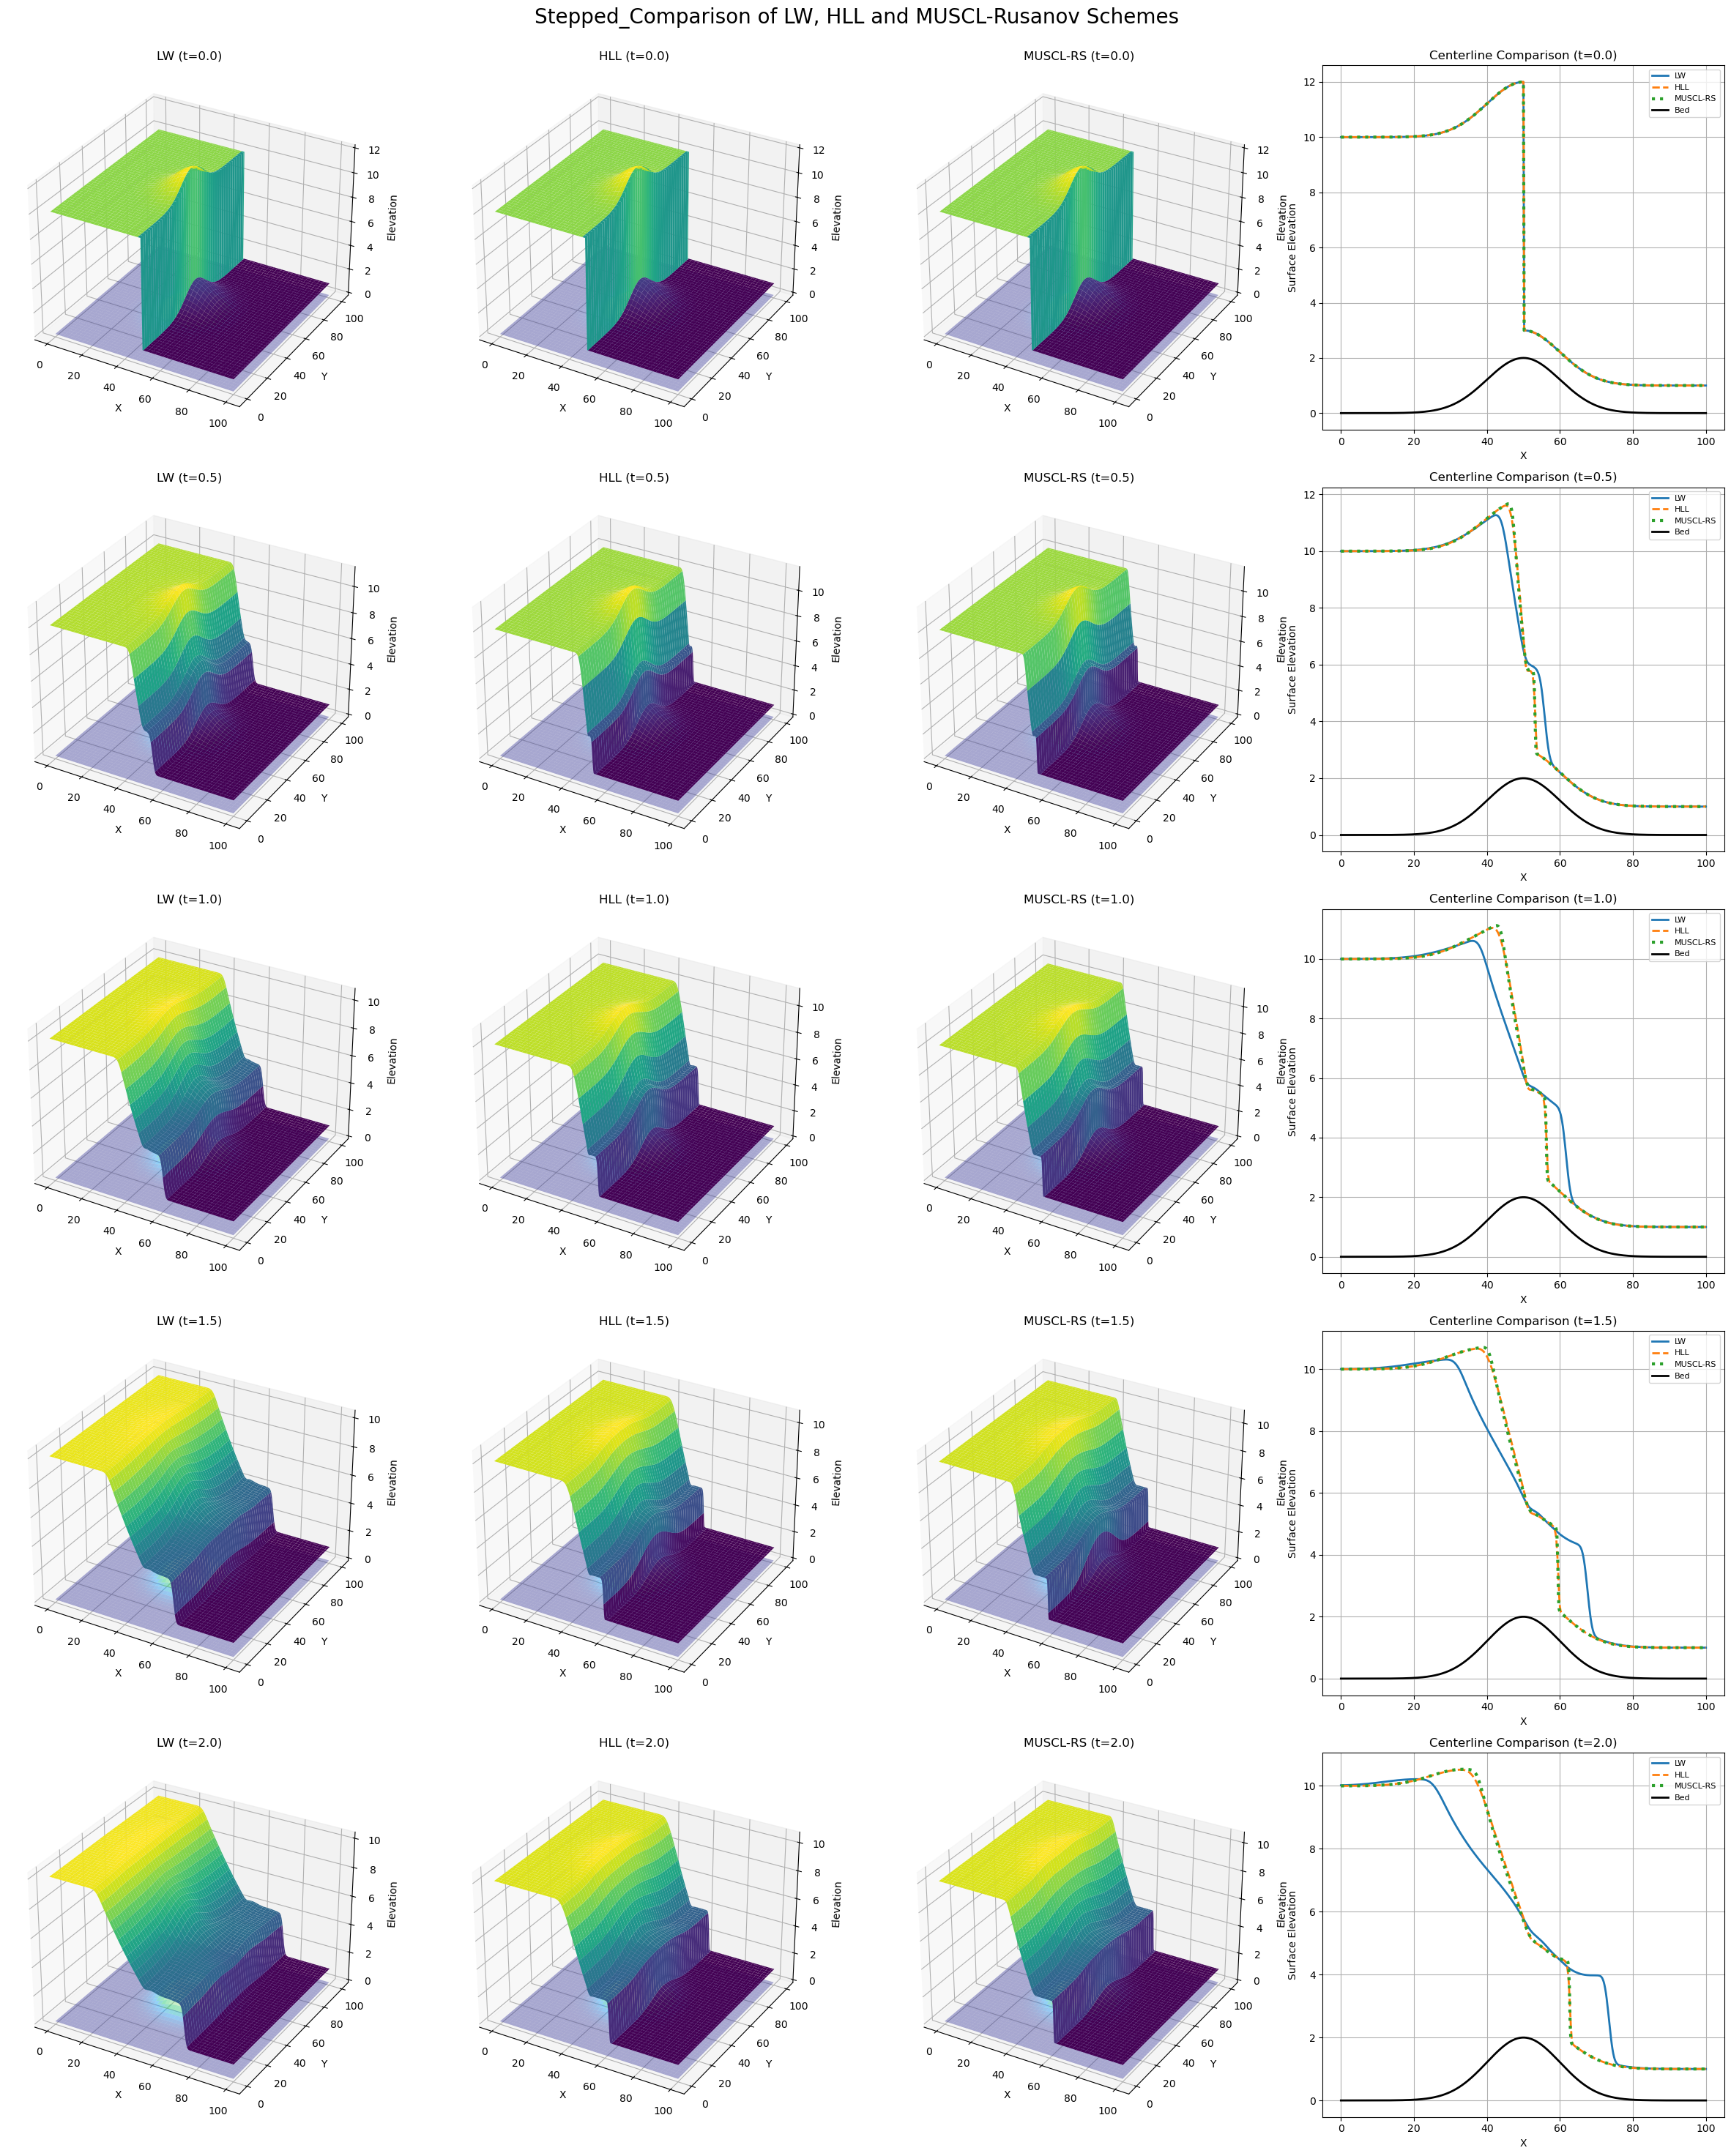
\includegraphics[width=\textwidth]{Step_Comparison_All_Times.png}
\caption{Comparison of the LW, HLL, and MUSCL--Rusanov schemes for the step dam-break problem at different time instances.}
\label{fig:step}
\end{figure}
\subsection{Variant 2: Rectangular Dam-Break}

The numerical solutions for the rectangular dam-break configuration are shown in figure~\ref{fig:rectangular}. In this situation, the water is first trapped in a rectangular area in the middle of the computational area. After the removal of the dam, the water flows out in all directions, resulting in multidirectional wave propagation and strong interactions in the corners of the reservoir.

Because of the interaction of waves at the edges and corners, these waves create complex structures in the rectangular geometry. All numerical schemes capture the overall spreading pattern, but there are discernible differences in the spreading near the discontinuities. The LW scheme is able to reproduce the growing fronts properly, while the regions with sharp gradients have oscillations. The HLL scheme produces stable and smooth solutions, but with a higher numerical diffusion. The MUSCL-Rusanov scheme provides a good solution and is able to keep the interface sharp and be numerically stable while giving a correct solution for the corner interactions.
\begin{figure}[H]
\centering
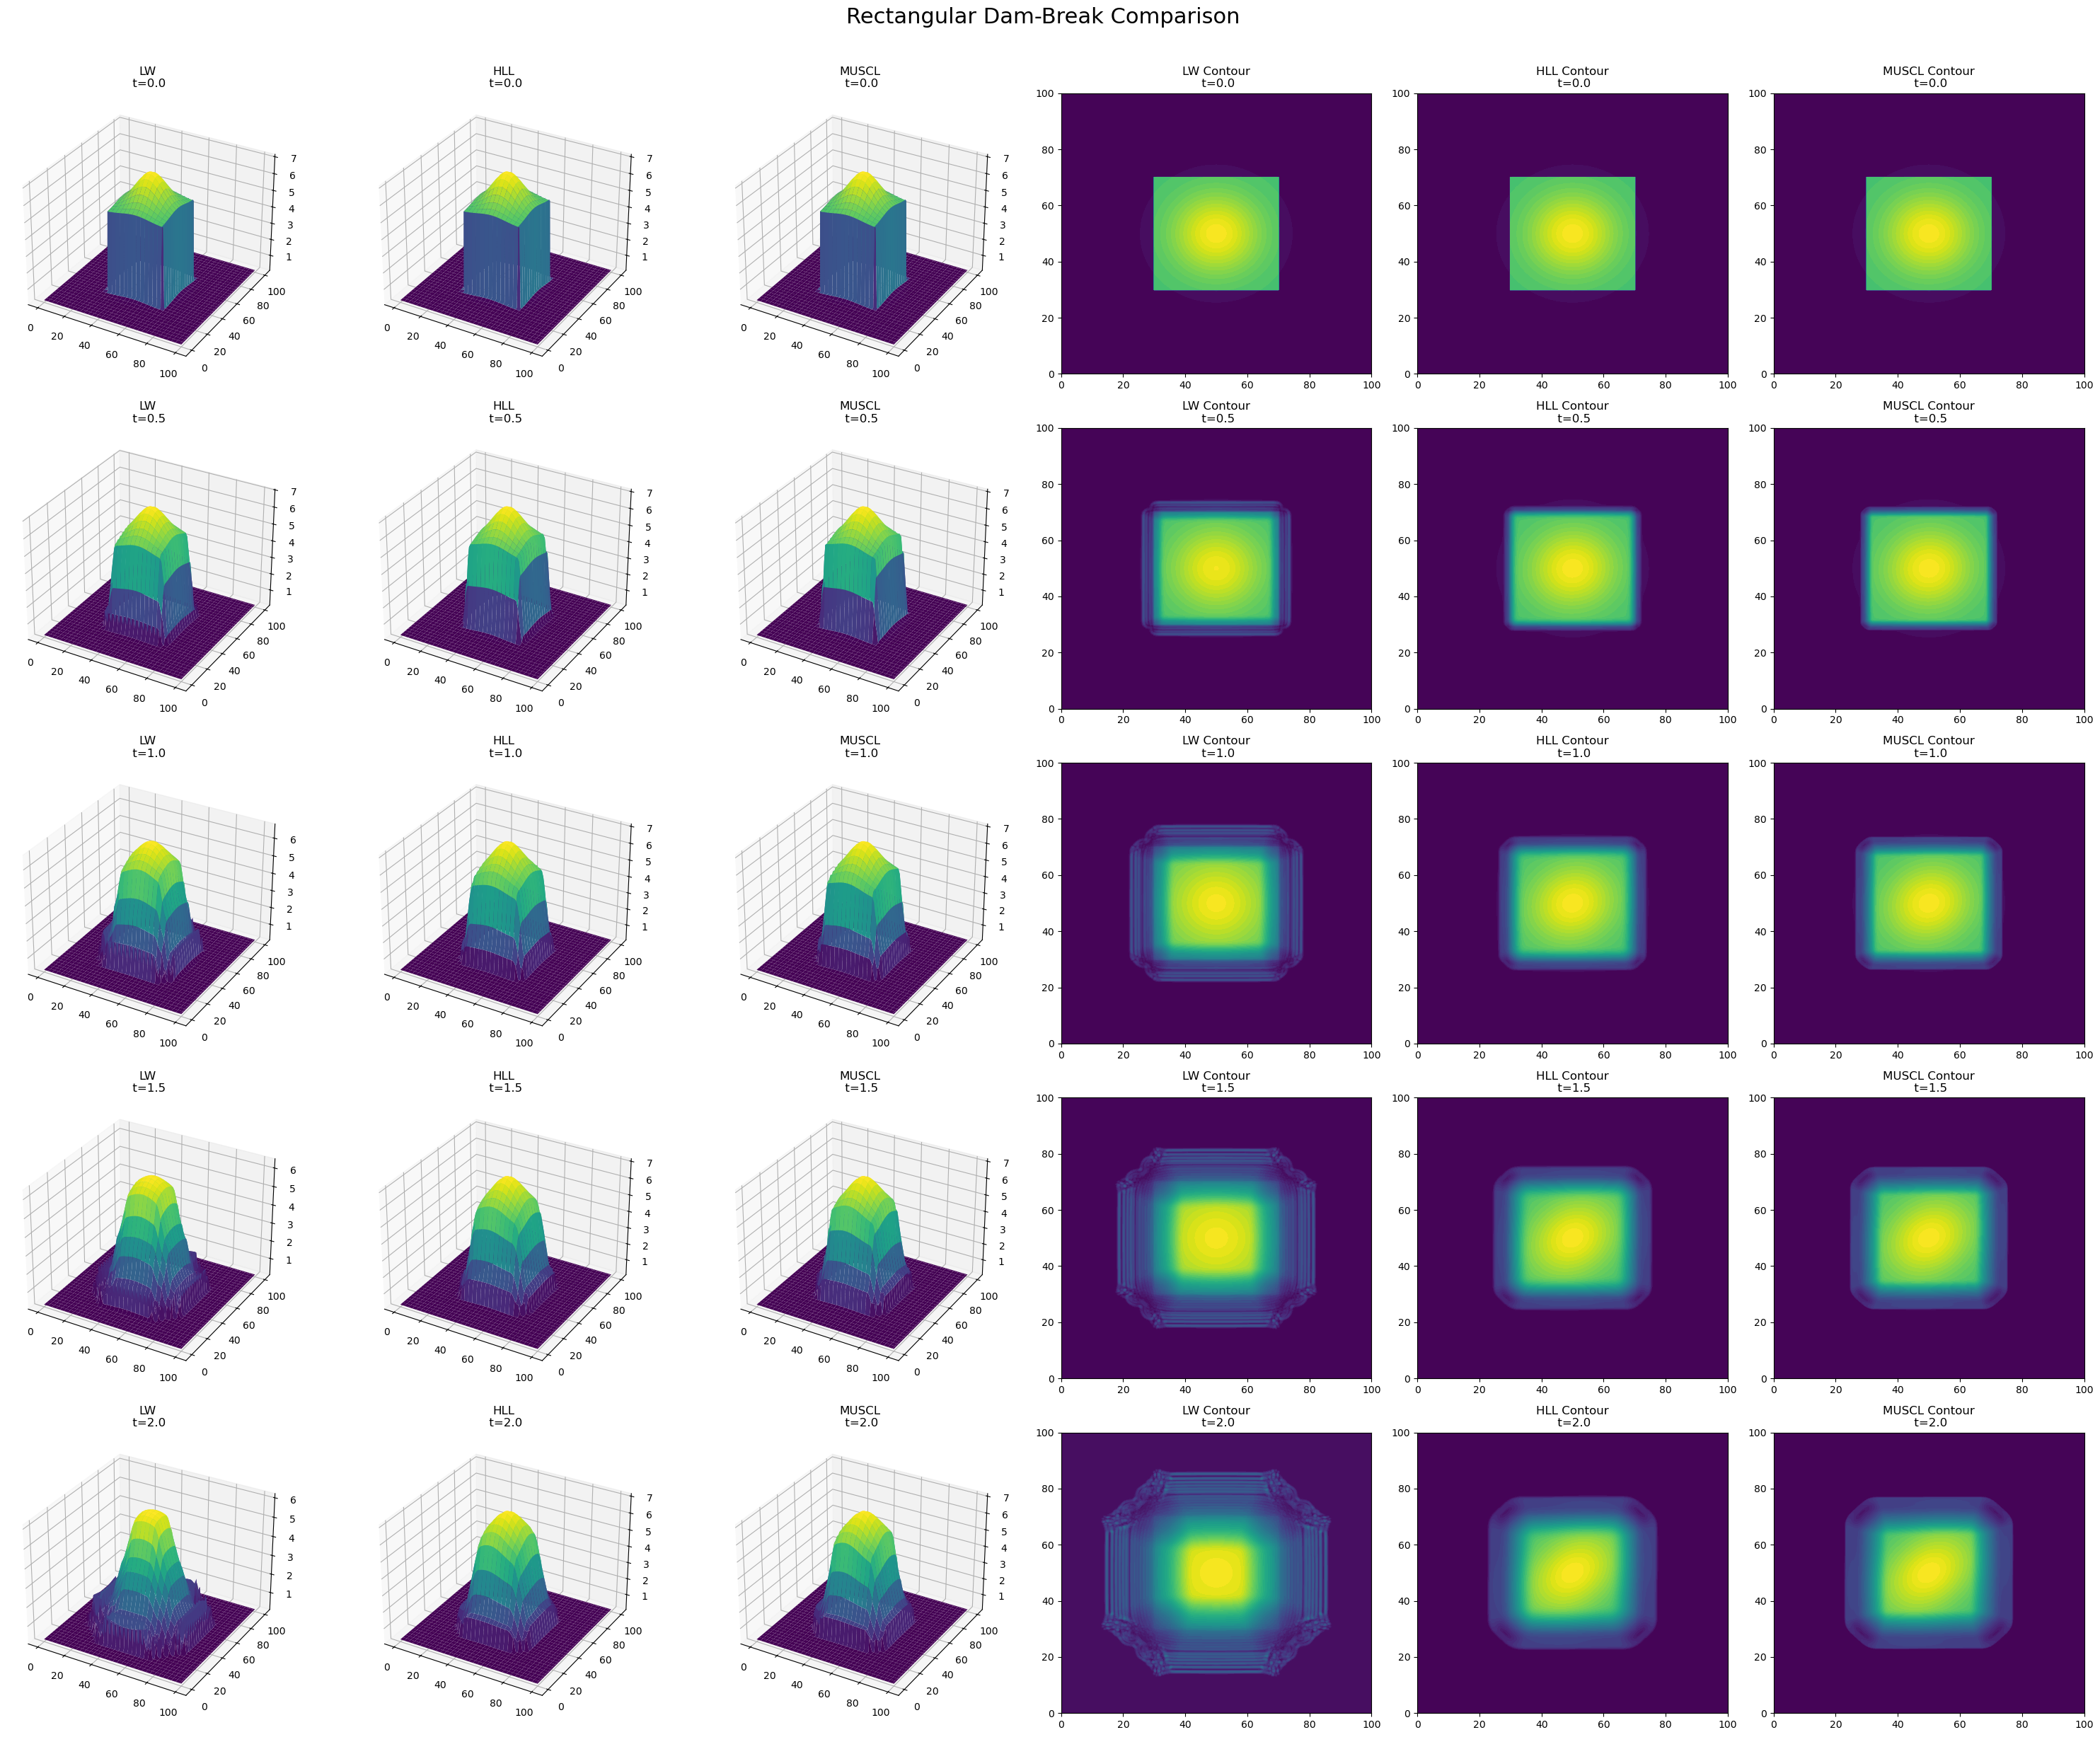
\includegraphics[width=\textwidth]{Rectangular_Comparison_All_Times.png}
\caption{Comparison of the LW, HLL, and MUSCL--Rusanov schemes for the Rectangular dam-break problem at different time instances.}
\label{fig:rectangular}
\end{figure}
\subsection{Variant 3: Circular Dam-Break}

The numeric solution results for the dam break problem with circular dams are displayed in Fig.~\ref{fig:circular}. The first water column that is confined to a cylinder is used as a source to set up radially symmetric waves that propagate outwards from the centre of the domain after the dam has been suddenly removed.

The overall radial symmetry of the flow is maintained during the simulation with all the numerical schemes. However, there are variations in the representation of the growing shock front. The LW scheme is able to accurately represent the propagating wave, but has some oscillations in the vicinity of the shock region. The HLL scheme is diffusive and hence gives smoother solutions. This is in contrast with the MUSCL--Rusanov scheme which is able to capture the shock front as well as maintain the radial symmetry and avoid the appearance of numerical oscillations. As a result, the MUSCL--Rusanov method is shown to perform better for circular wave propagation.
\begin{figure}[H]
\centering
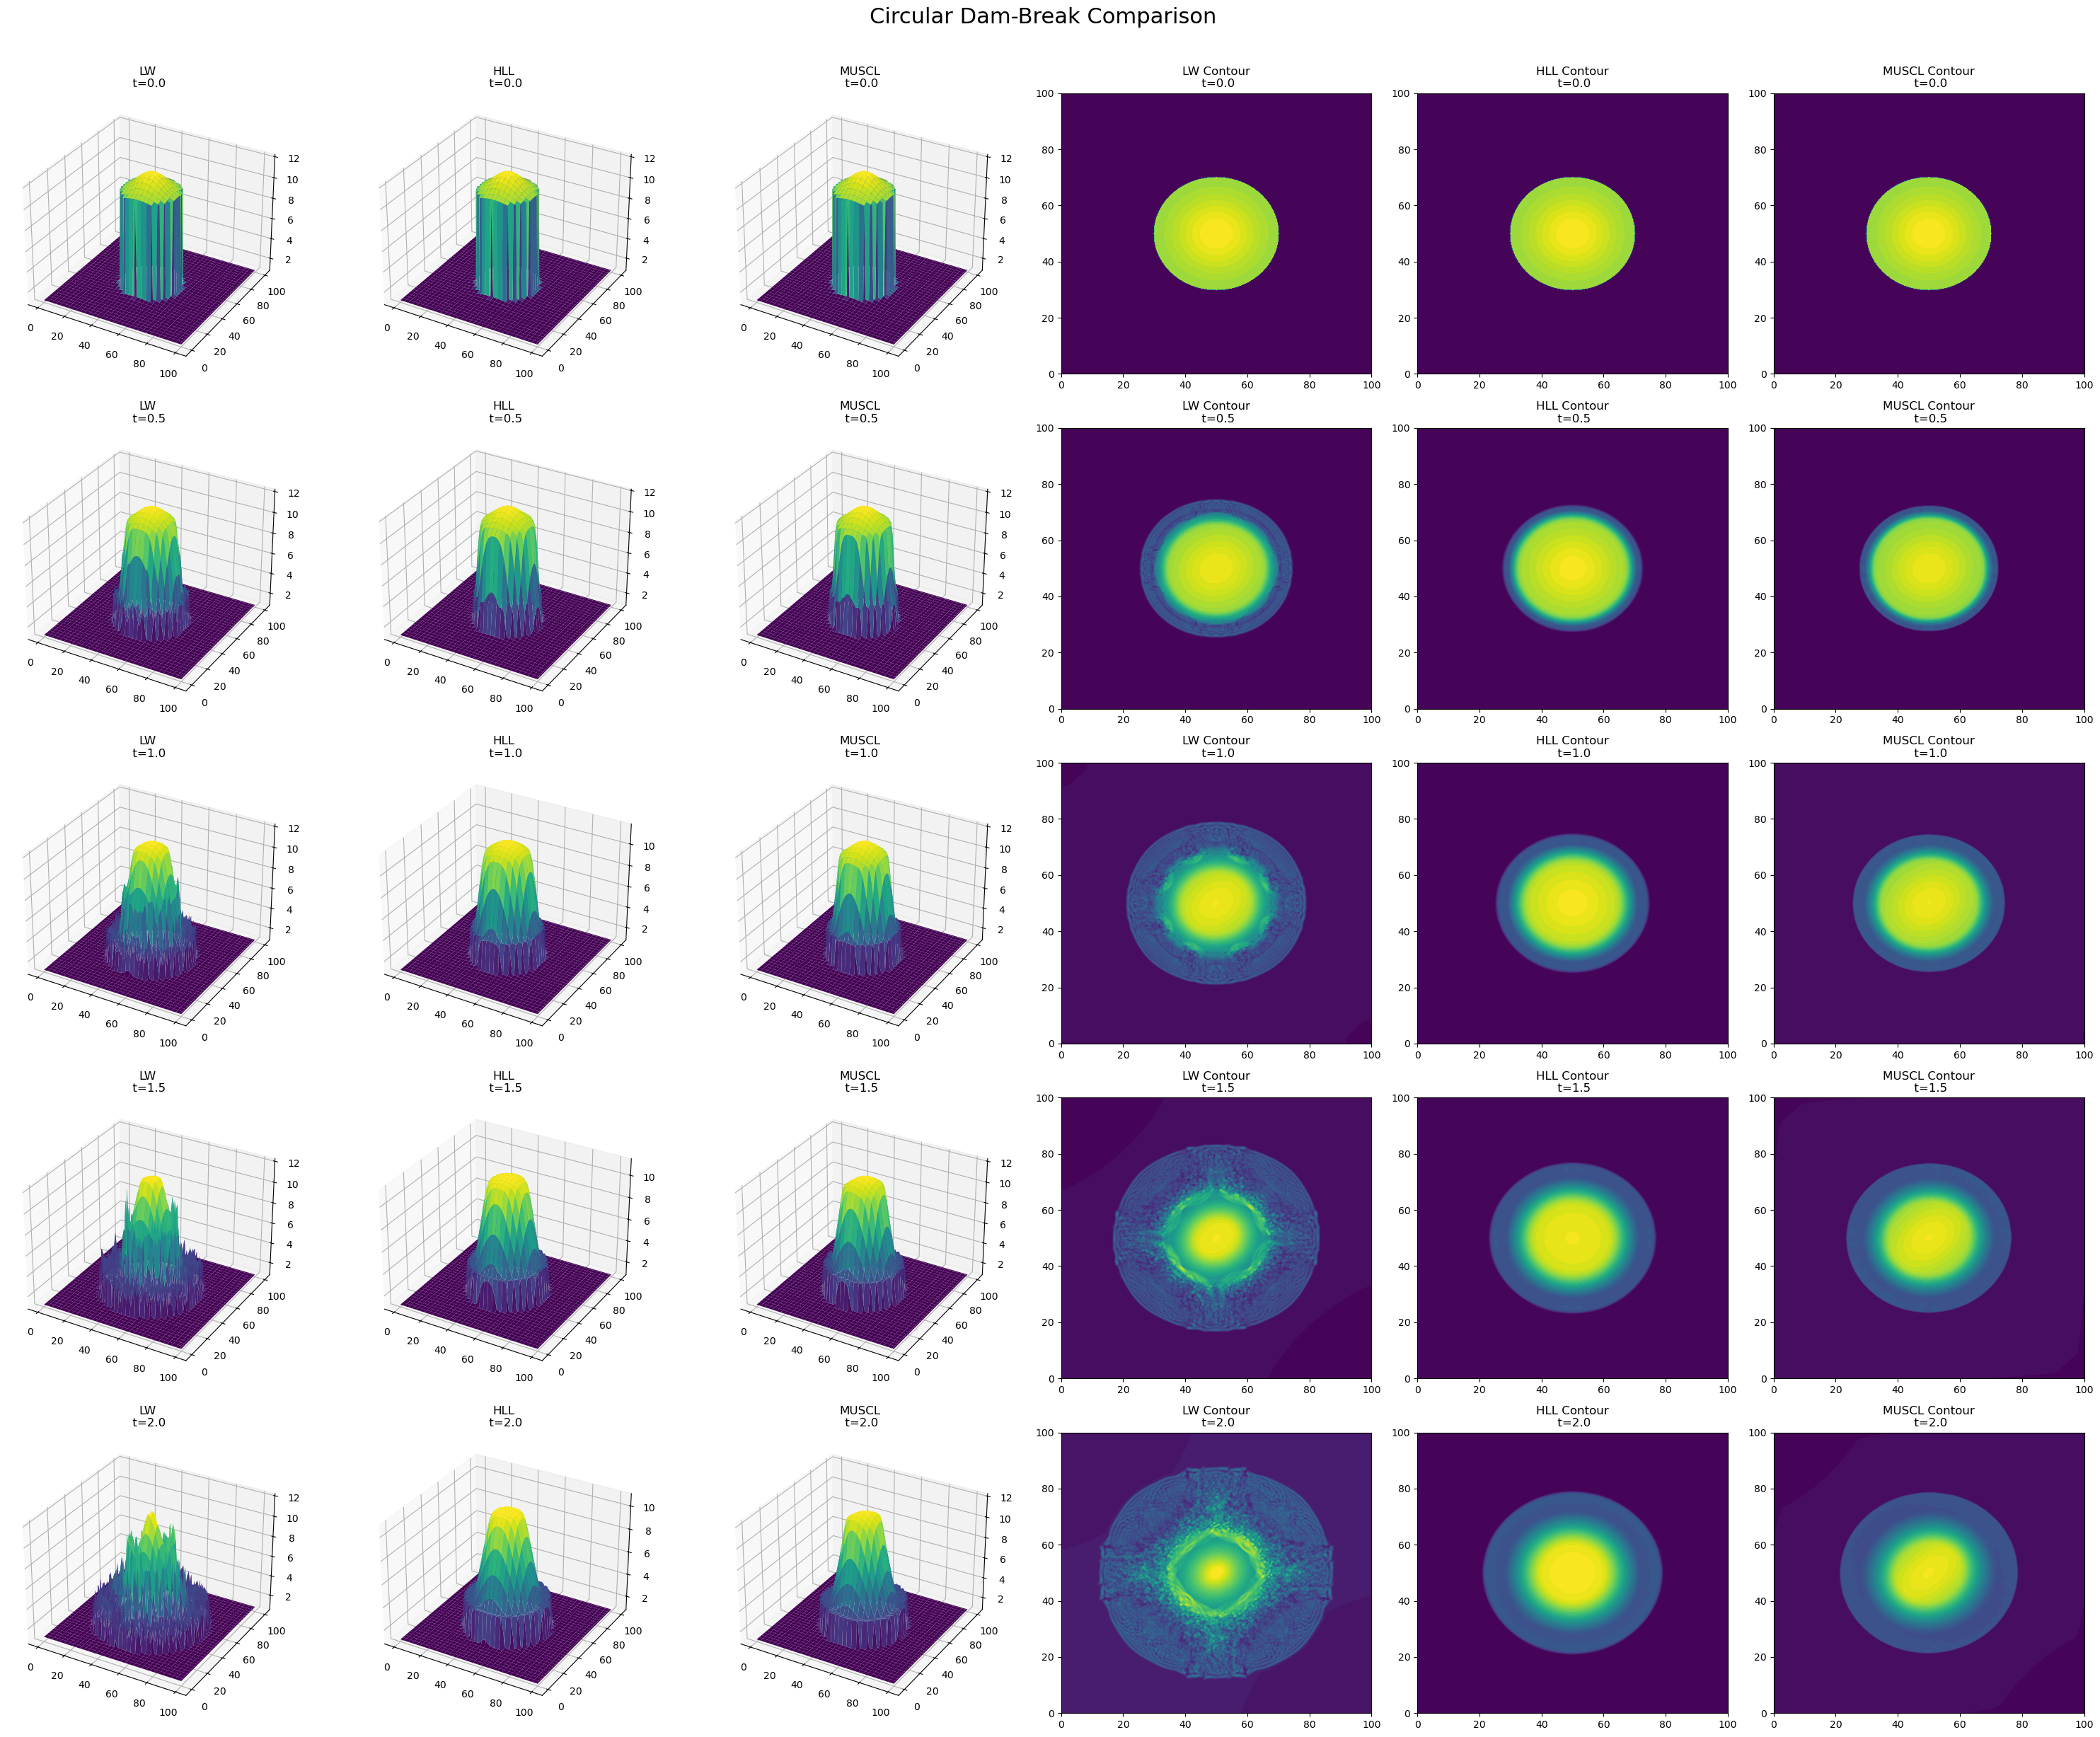
\includegraphics[width=\textwidth]{Circular_Comparison_All_Times.png}
\caption{Comparison of the LW, HLL, and MUSCL--Rusanov schemes for the Circular dam-break problem at different time instances.}
\label{fig:circular}
\end{figure}
\subsection{Variant 4: Gaussian Dam-Break}

The time evolution of the Gaussian dam-break configuration is shown in Figure~\ref{fig:gaussian}. In contrast to the previous discontinuous cases, the Gaussian initial condition is a smooth free surface profile, with a continuous water depth distribution.

There are no initial sharp discontinuities and all three numerical schemes produce good results and retain the smoothness of the propagating wave. The LW scheme is highly accurate but can give some dispersive effects in a long time integration. The HLL scheme shows no change in the stability of the scheme during the simulation, but there is a little bit of numerical diffusion. The MUSCL--Rusanov scheme is able to preserve the amplitude and the shape of the Gaussian profile better, and thus the smooth flow evolution is best represented by this scheme.
\begin{figure}[H]
\centering
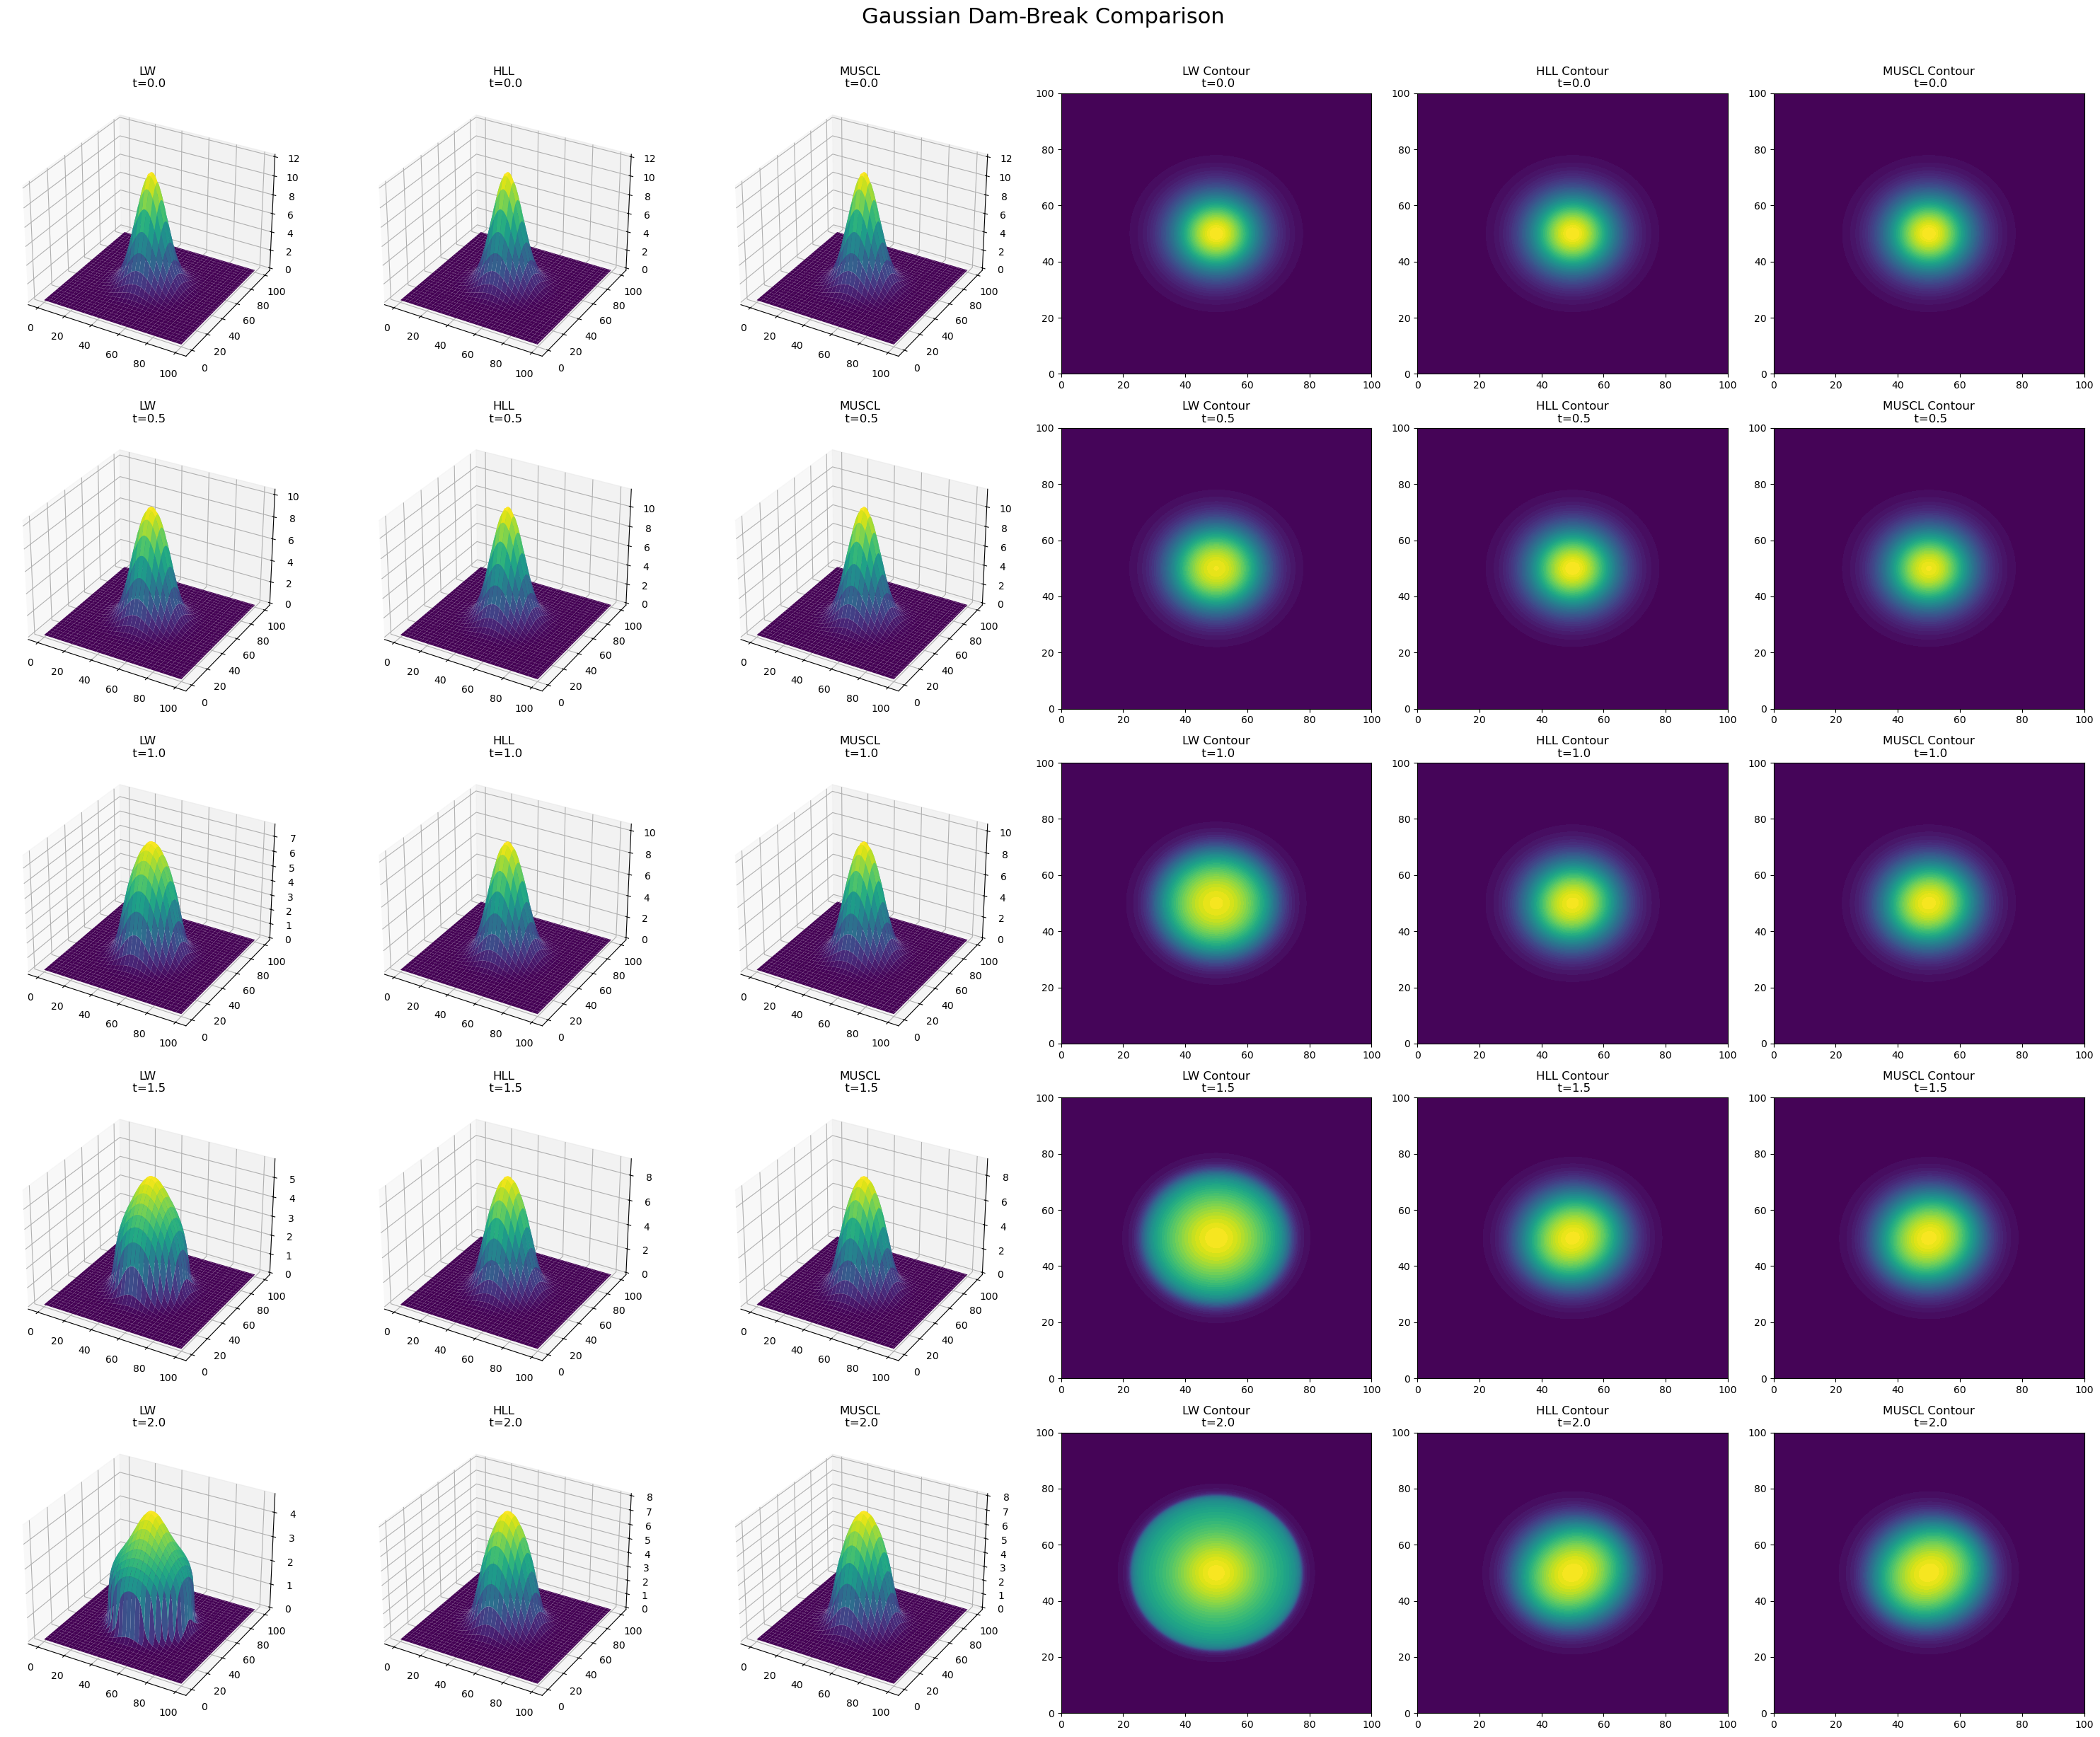
\includegraphics[width=\textwidth]{Gaussian_Comparison_All_Times.png}
\caption{Comparison of the LW, HLL, and MUSCL--Rusanov schemes for the Gaussian dam-break problem at different time instances.}
\label{fig:gaussian}
\end{figure}
\subsection{Variant 5: Parabolic Dam-Break}

In figure \ref{fig:parabolic} numerical solution to the parabolic dam-break problem is shown. The underlying bed topography has a complex relationship with the water profile, the propagation patterns are not uniform, and are curved in the first water profile.

This curved boundary creates asymmetric patterns in the flow, which also results in changes in the wave speed at certain points. All schemes are able to reproduce the dominant hydrodynamic features, but the LW scheme shows oscillatory behaviour in the region of the steep gradients. The HLL scheme is stable, but the propagating wave fronts tend to smear, because of numerical diffusion. The MUSCL--Rusanov scheme, on the other hand, preserves the curved interfaces correctly and has excellent stability and stability minimizing spurious oscillations. The results presented here validate the robustness of the MUSCL--Rusanov scheme on the geometrically complex flow configurations.
\begin{figure}[H]
\centering
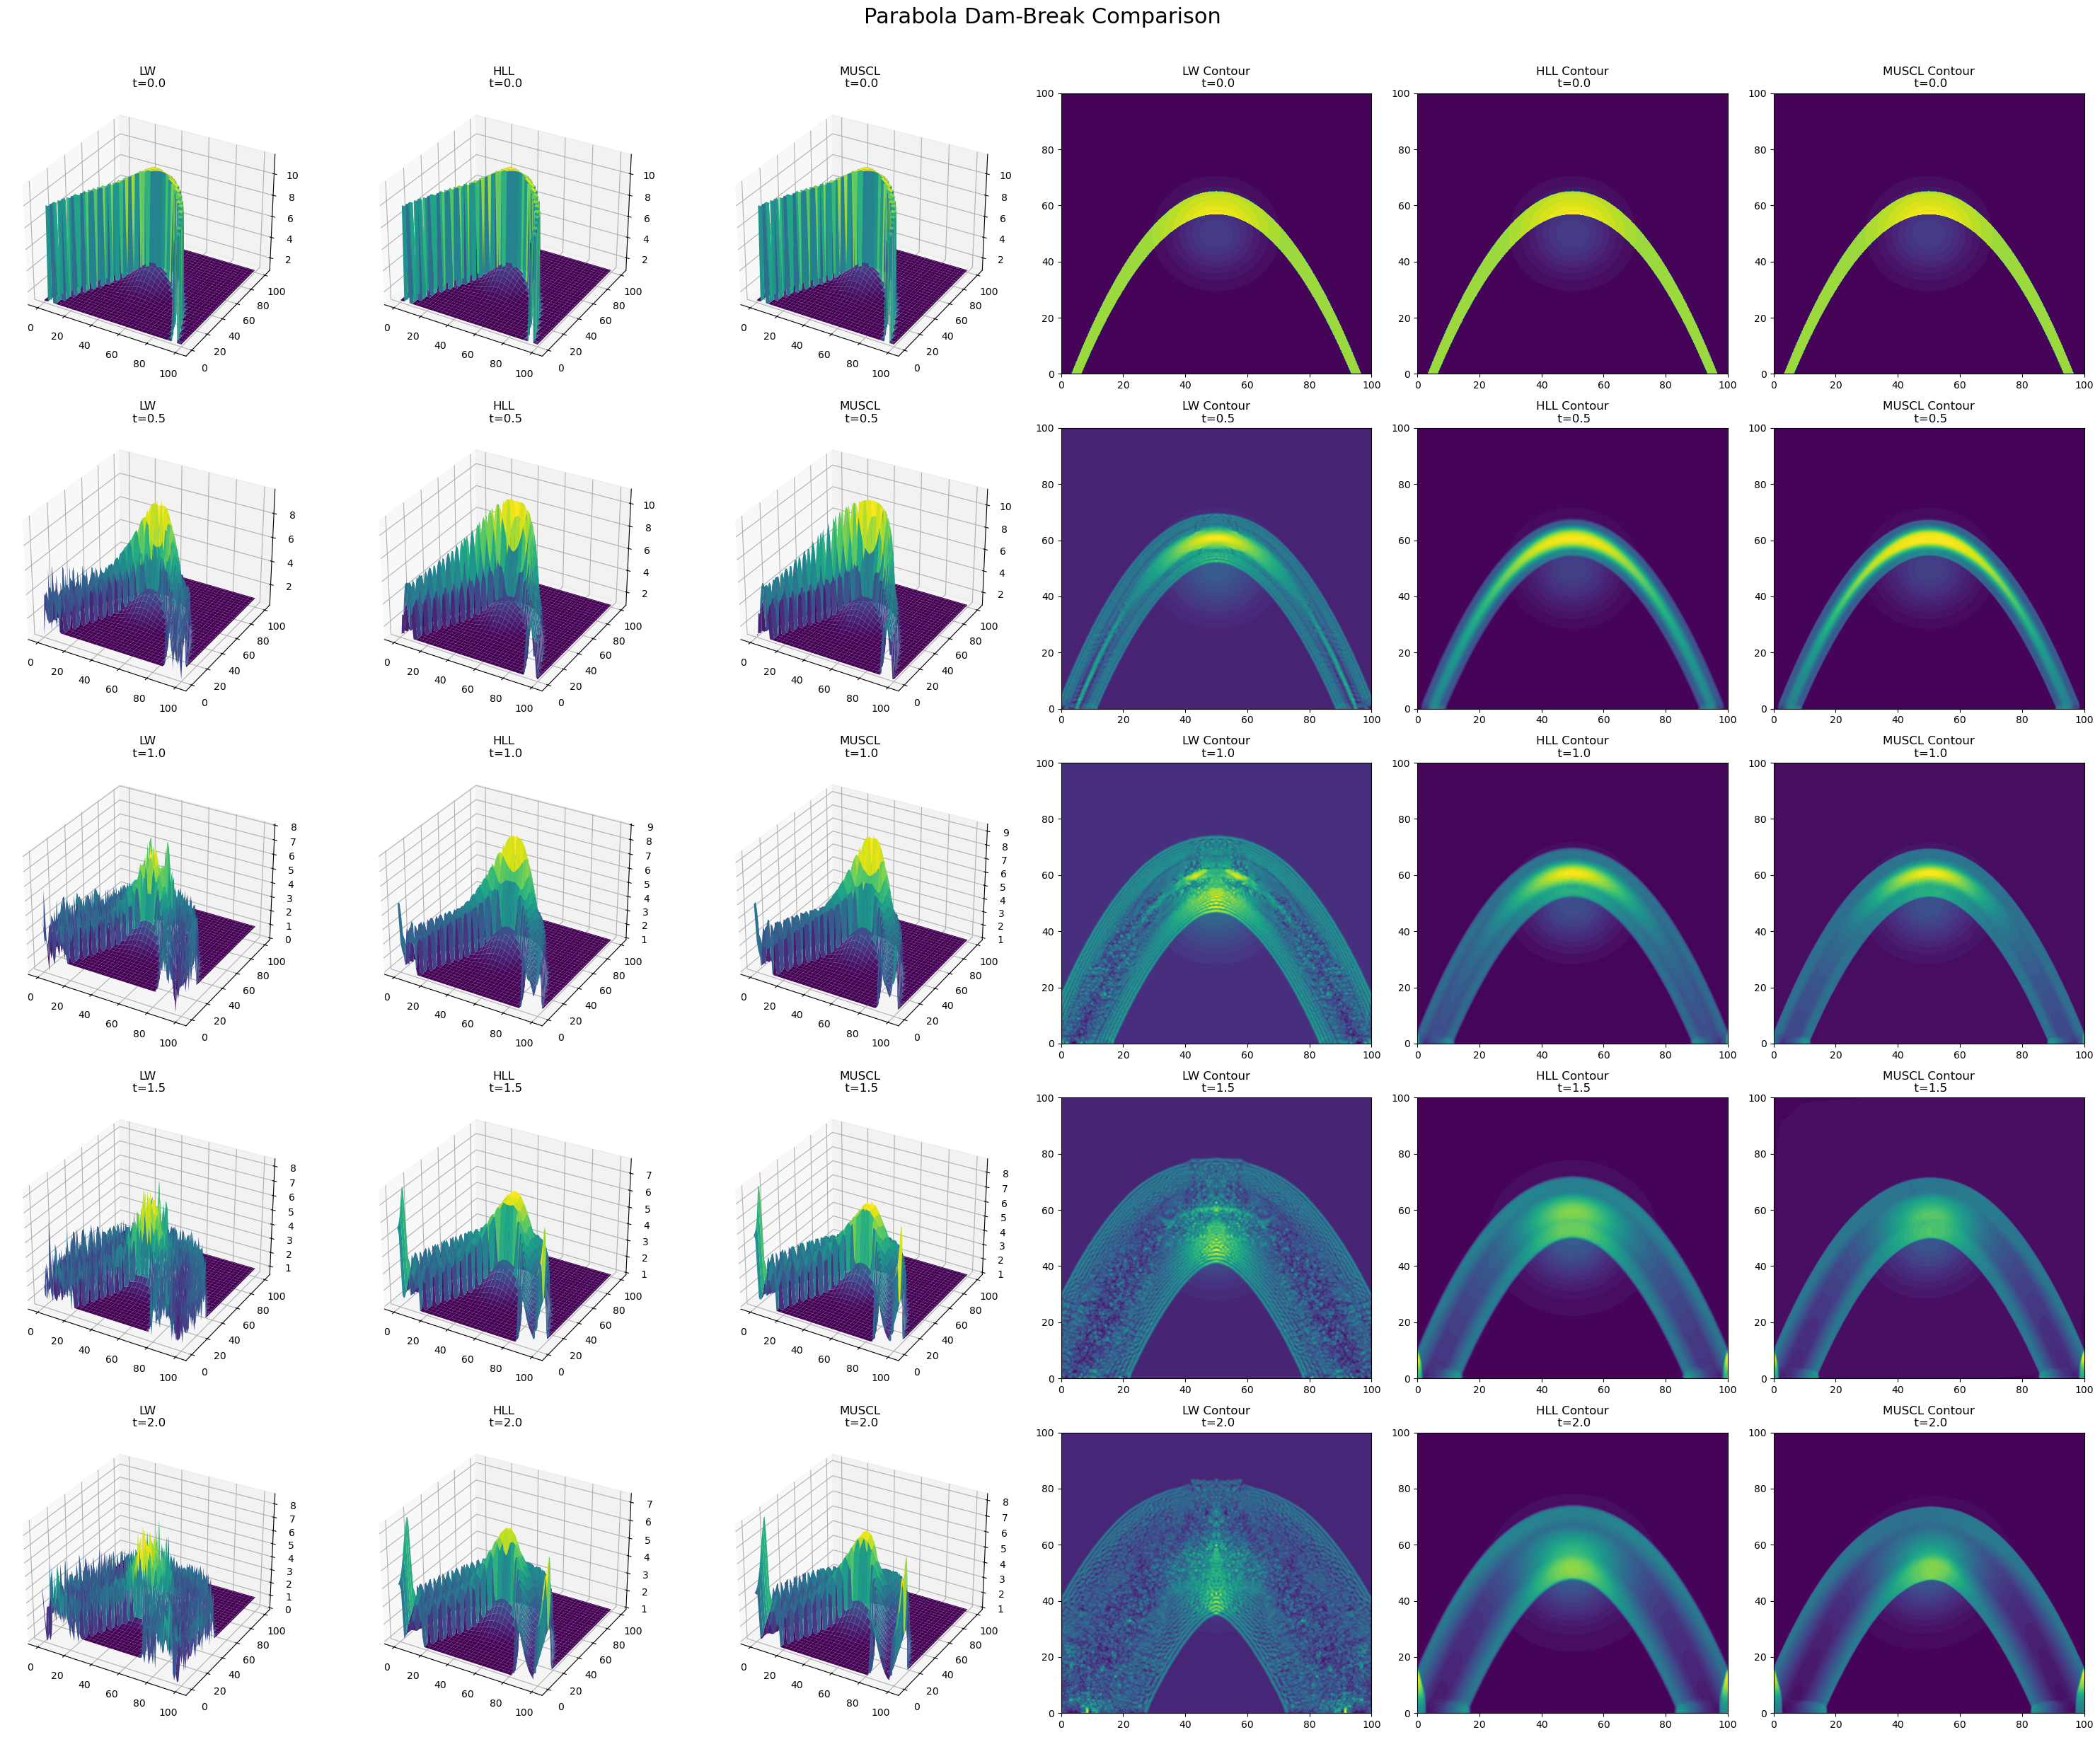
\includegraphics[width=\textwidth]{Parabola_Comparison_All_Times.png}
\caption{Comparison of the LW, HLL, and MUSCL--Rusanov schemes for the Parabola dam-break problem at different time instances.}
\label{fig:parabolic}
\end{figure}
\subsection{Variant 6: Triangular Dam-Break}

The numerical results for the triangular dam-break configuration are shown in figure~\ref{fig:triangular}. This benchmark problem is complicated by sharp vertices and tilted boundaries, which produce complex interactions of the waves and strong shock reflections.

The propagating waves that come from the triangular vertices interact with each other and form complex flow structures throughout the computational domain. The LW scheme clearly reproduces these interactions, but there are discontinuities and noticeable oscillations near the vertices. This HLL scheme successfully suppresses oscillations but results in relatively broad wave fronts. The MUSCL--Rusanov scheme is accurate in solving the corner interactions and retains the overall triangularity of the solution with the stability of the numerical solution. Overall, the MUSCL--Rusanov scheme is the most accurate and stable for the triangular dam-break problem.
\begin{figure}[H]
\centering
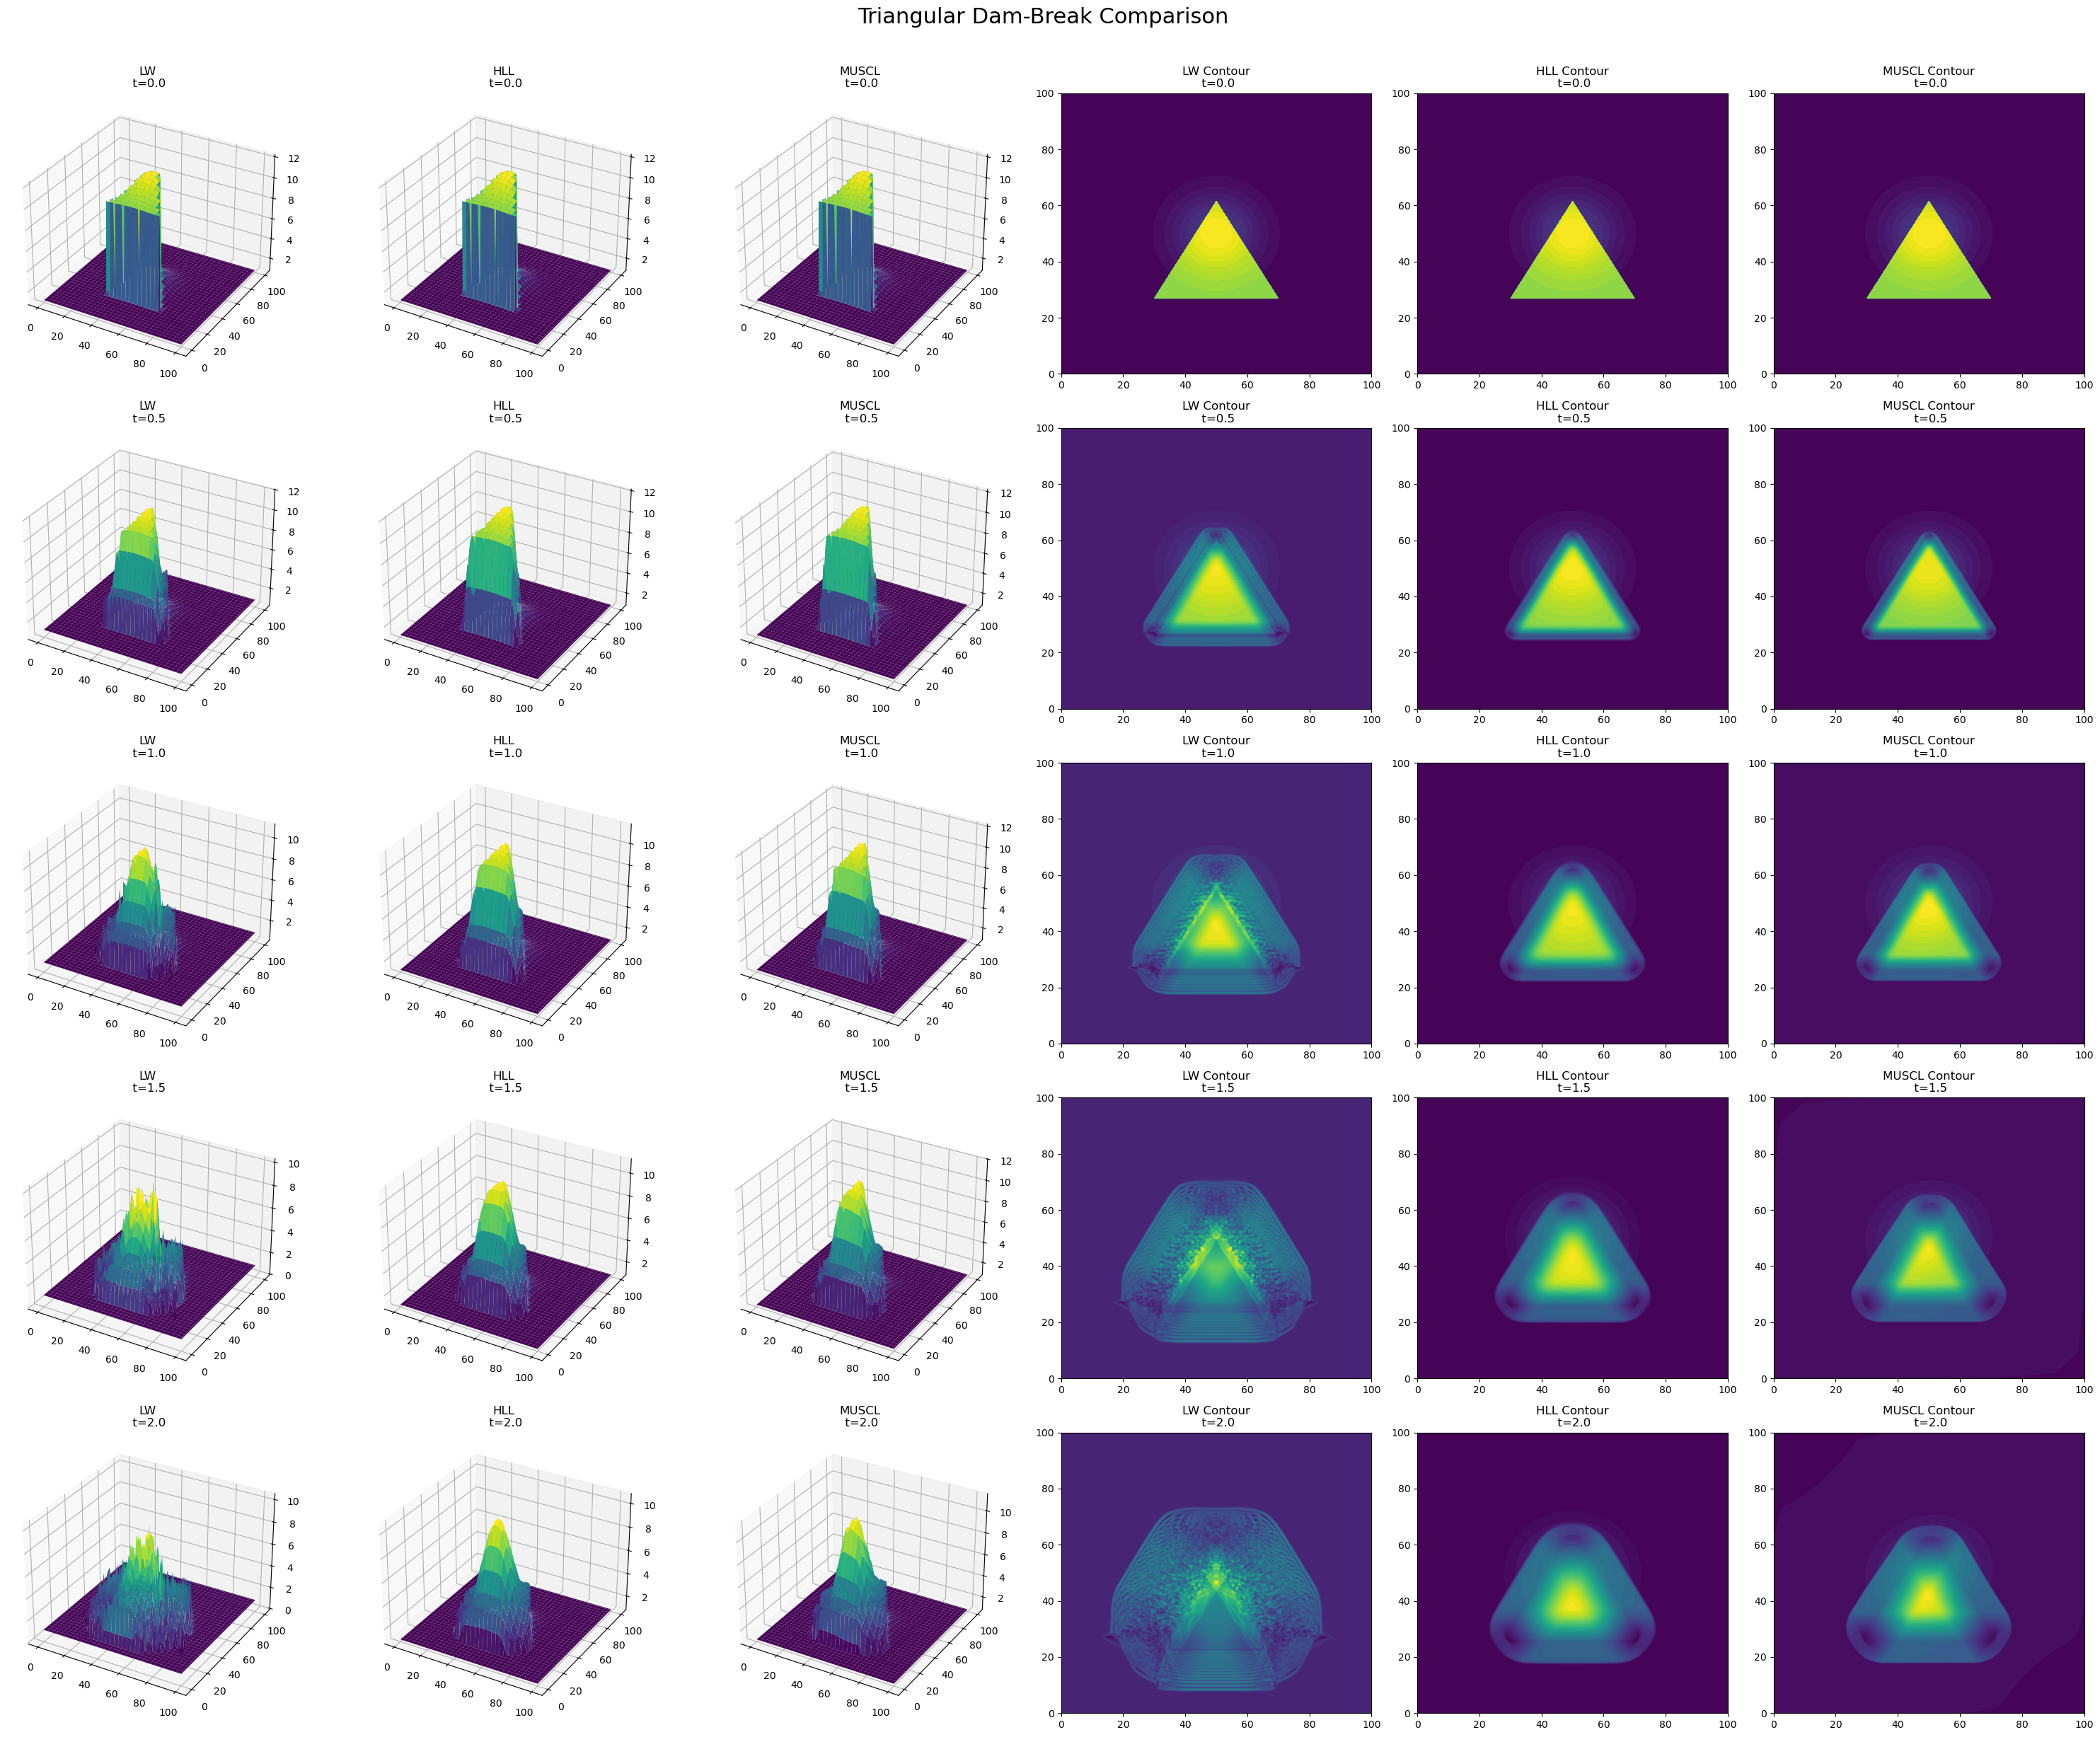
\includegraphics[width=\textwidth]{Triangular_Comparison_All_Times.png}
\caption{Comparison of the LW, HLL, and MUSCL--Rusanov schemes for the Triangular dam-break problem at different time instances.}
\label{fig:triangular}
\end{figure}

\begin{newtext}
% ---- SCAFFOLD (new, in red): SciML comparison results. All numbers, figures,
% and tables below are placeholders pending completion of the training runs.
\subsection{SciML Comparison}

This section compares the strong-form PINNs (primitive and conservative) and the FVM--PINN against the reference solutions of Sect.~4.1--4.6. [PENDING: results from the full training runs; the structure below is fixed, the content is placeholder.]

\subsubsection{Accuracy against reference solutions}

[TABLE: per-variant $L^1$/$L^2$ errors of $h$ and velocity magnitude at $t=2.0$~s for PINN (primitive), PINN (conservative), and FVM--PINN, mean $\pm$ std over three seeds. One row per initial-condition variant.]

[FIGURE: side-by-side depth contours at $t=1.0$ and $t=2.0$~s -- reference (MUSCL--Rusanov) vs.\ PINN vs.\ FVM--PINN -- for the Step and Circular variants, with centerline profiles highlighting shock smearing.]

Expected discussion points once results are in: (i) whether the conservative formulation reduces error relative to the primitive formulation near shocks, as the weak-solution argument predicts; (ii) how error scales with the geometric complexity of the initial condition (smooth Gaussian vs.\ discontinuous step/circular vs.\ cornered rectangular/triangular); (iii) where in the domain the error concentrates (shock and rarefaction fronts, as reported by \cite{tian2025pinnswe,mumtaz2025dambreak}).

\subsubsection{Conservation}

[FIGURE/TABLE: relative mass drift over time for each model and variant, against the machine-precision conservation of the finite-volume schemes and the documented drift of the LW scheme.]

\subsubsection{Shock-front position}

[TABLE: front-position error at each output time for the Step (planar front) and Circular (radial front) variants.]

\subsubsection{Data-guidance ablation}

[TABLE/FIGURE: FVM--PINN and PINN errors with and without sparse observations injected into the loss, testing whether the zero-momentum collapse reported in \cite{liu2026fvmpinn} occurs in this setting and how many observation points are needed to prevent it.]

\subsubsection{Computational cost}

[TABLE: training time, inference time for the full space-time solution, and classical-scheme runtime on the same hardware (CPU and GPU).]
\end{newtext}

\begin{newtext}
% ---- SCAFFOLD (new, in red): Discussion.
\section{Discussion}

[TODO: write after results. Planned argument structure:]
\begin{itemize}
  \item \textbf{Where classical schemes remain superior.} Accuracy per unit cost at shocks; exact conservation; robustness across all six initial-condition geometries without retraining or tuning.
  \item \textbf{What the neural formulations buy.} Mesh-free space-time representation, differentiability with respect to inputs and parameters, and the amortization argument (inference cost after training); honest accounting of training cost against a single solver run.
  \item \textbf{Primitive vs.\ conservative PINN.} Interpret the observed differences through the weak-form/Rankine--Hugoniot lens.
  \item \textbf{Discrete vs.\ strong-form residuals.} Whether the FVM--PINN's solver-consistency loss narrows the gap at discontinuities and in mass conservation, and the cost of evaluating the residual through solver steps.
  \item \textbf{Sensitivity to initial dam-breaking conditions.} Which geometries are hardest for each method family, and why (corner interactions, radial symmetry preservation, smooth vs.\ discontinuous data).
  \item \textbf{Limitations.} Single-instance training (no generalization across scenarios -- contrast with operator learning \cite{lu2021deeponet,li2021fourier}); idealized setting ($n=0$, wet bed, reflective walls, $g=2$~m/s$^2$); grid-bound reference solutions.
\end{itemize}
\end{newtext}

\begin{newtext}
% ---- SCAFFOLD (new, in red): Conclusion.
\section{Conclusion}

[TODO: write after results. Planned content: restate the benchmark matrix (six initial-condition geometries $\times$ three classical schemes $\times$ three neural formulations over a Gaussian-hump bed); summarize the classical-scheme ranking (MUSCL--Rusanov best overall, HLL most robust but diffusive, LW oscillatory near steep gradients); summarize the SciML findings once available; state the main takeaway on when physics-informed networks are and are not competitive for dam-break simulation; outline future work -- operator-learning extensions for cross-scenario generalization \cite{li2024pino,wang2026lgno}, wet/dry fronts, friction and rainfall source terms, and real-topography case studies.]
\end{newtext}

\bibliographystyle{unsrt}
\bibliography{references}

\end{document}